% Template by Falko Galperin <falko1@tzi.de>, 2022, V1.0
% Main styling of the template comes from the ClassicThesis package by André Miede.

% IMPORTANT POINTS BELOW:
% - Look at the options between "CONFIGURATION HERE" and "CONFIGURATION ENDS".
% - Abstract.tex contains the abstract (can be disabled).
% - Inhalt.tex contains the contents of your thesis.
% - Glossar.tex contains the glossary (can be disabled) and further options.

% Less important points:
% - You can compile a PDF using `make` and clean up unnecessary files 
%   using `make clean`. `make pdf` combines both.
% - CMYK color space will be used so that printers don't get confused.
% - Feel free to configure other parts outside of the section below too,
%   e.g. uncomment the list of tables if you want that.

%%% CONFIGURATION HERE %%%

% Enter information about your thesis here, adjust as necessary.
% I recommend keeping the `\xspace` at the end.
\newcommand{\myTitle}{System porting to mobile devices at the example of the SEE project\xspace}
\newcommand{\mySubtitle}{Master Thesis\xspace}
\newcommand{\myName}{Roman Gressler\xspace}
\newcommand{\myNumber}{3217822\xspace}
\newcommand{\myProf}{Prof.\ Dr.\ Rainer Koschke\xspace}
\newcommand{\myOtherProf}{Dr.\ Robert Porzel\xspace}
\newcommand{\myDepartment}{Faculty 3 --- Mathematics and Computer Science\xspace}
\newcommand{\myDegree}{Computer Science\xspace}
\newcommand{\myDate}{\today}
\newcommand{\myVersion}{\classicthesis}

% Whether links should be colored.
\def\colorLinks{true}

% Color for citations.
\def\citeColor{Periwinkle}

% Color for URLs.
\def\urlColor{Cyan}

% The file in which your BibLaTeX sources reside.
% Remove this line to disable the bibliography.
\def\sourcesFile{sources.bib}

% If you won't use the glossary template, remove the following line.
% Otherwise, set this to the filename of the glossary LaTeX file.
\def\glossaryFile{Glossar.tex}

% If you don't want to have an abstract, remove the following line.
% Otherwise, set this to the filename of the LaTeX file containing the abstract.
\def\abstractFile{Abstract.tex}

% Despite the seemingly broad implications of this option, it'll simply include a 
% disclaimer for readers in case you don't want to use something 
% like the "Gendersternchen". Set it to 1 to enable this disclaimer.
\def\disableGender{0}

% Set this to 1 if you want to use \section for the highest level of headings.
% Otherwise, \chapter will be used.
% IMPORTANT NOTE: This template assumes this value will be 1.
% If you choose to set it to something other than 1, you'll need to
% adjust this template's usage of \section and change it to \chapter.
\def\disableChapter{1}

% These are ClassicThesis options. 
% Don't forget to set drafting=false for the final version.
% If you have pdflatex, I recommend eulermath=true, it looks a bit better in my opinion.
\PassOptionsToPackage{
  drafting=true,  % print version information on the bottom of the pages
  tocaligned=false, % the left column of the toc will be aligned (no indentation)
  dottedtoc=true,  % page numbers in ToC flushed right
  eulerchapternumbers=true, % use AMS Euler for chapter font (otherwise Palatino)
  linedheaders=false,  % chaper headers will have line above and beneath
  floatperchapter=true,  % numbering per chapter for all floats (i.e., Figure 1.1)
  eulermath=false,  % use Euler fonts for mathematical formulae (only with pdfLaTeX)
  beramono=true,    % toggle a different monospaced font (w/ bold)
  style=classicthesis % classicthesis, arsclassica
}{classicthesis}

%%% CONFIGURATION ENDS %%%
% (Of course, feel free to modify the rest of the below code too.)

% ClassicThesis causes these false positive warnings, hence we silence them.
\RequirePackage{silence} % :-\
    \WarningFilter{scrreprt}{Usage of package `titlesec'}
    \WarningFilter{titlesec}{Non standard sectioning command}

\documentclass[twoside,openright,titlepage,numbers=noenddot,%headlines,
               headinclude,footinclude,cleardoublepage=empty,abstract=on,
               BCOR=5mm,paper=a4,listof=totocnumbered]{scrreprt}
\usepackage[utf8]{inputenc}
\usepackage[T1]{fontenc}

\PassOptionsToPackage{hyphens}{url}

\usepackage[english]{babel}
\usepackage[dvipsnames,usenames,cmyk, table]{xcolor}
\usepackage{hyperref} 
\usepackage{xspace}
% \usepackage[style=alphabetic]{biblatex}
\usepackage[round]{natbib} % Literatur und Referenzen
\usepackage{bm}
\usepackage{dsfont}
\usepackage{sidenotes}
\usepackage{newpxtext}
\usepackage{epigraph}
\usepackage{etoolbox}
\usepackage{multicol}
\usepackage{graphicx}
\usepackage{wrapfig}
\usepackage{microtype}
% Note: If you enable this, you need the -shell-escape flag.
%\usepackage{minted}
%\usemintedstyle{friendly}
\usepackage{xifthen}
\usepackage{enumitem}
\usepackage{calc}
\usepackage{subfig}
\usepackage{amssymb}
\usepackage{scalerel}
\usepackage[noend]{algpseudocode}
\usepackage{algorithm}
\usepackage{xstring}

\usepackage[normalem]{ulem}
\setlength{\columnsep}{0,1cm}

\usepackage{classicthesis}
\usepackage{titlesec}
\usepackage{multirow}
\usepackage{graphicx}
\usepackage{rotating}
\usepackage{tikz}
\usepackage{sidecap}
\usepackage{listings}
% Make headings a little more discernable.
\titleformat*{\chapter}{\LARGE\bfseries}
\titleformat*{\section}{\Large\bfseries}
\titleformat*{\subsection}{\large\bfseries}

\hypersetup{colorlinks=\colorLinks, citecolor=\citeColor, 
    urlcolor=\urlColor, linktocpage=true, bookmarksnumbered,
  pdftitle={\myTitle},%
  pdfauthor={\textcopyright\ \myName, University Bremen},%
  pdfsubject={\mySubtitle},%
  pdfcreator={pdfLaTeX},%
  pdfproducer={LaTeX with classicthesis and FG-V1.0}%
}

%\ifdef{\sourcesFile}{\addbibresource{\sourcesFile}}{}

% Allow " instead of "` and "'
\usepackage{csquotes}
\MakeOuterQuote{"}

% Uncomment this if you want textsc to be a little (x 1.15) bigger.
%\usepackage{letltxmacro,scalefnt}
%\newcommand{\bigtextsc}[1]{\textsc{\scalefont{1.15}#1}}

% Some custom commands:
% Proper spacing for "z.B."
\newcommand{\zB}{z.\,B.\xspace}
% Command for TODOs, use either \TODO or \TODO{Details}
\newcommand{\TODO}[1]{\textbf{\textcolor{red}{\ifthenelse{\isempty{#1}}{TODO!}{TODO: #1}}}\xspace}
% Properly color Axivion's name.
\newcommand{\Axivion}{\textsc{{\color{black}{A}}{\color{red}{x}}{\color{black}{ivion}}}}

\newcommand{\Regie}[1]{\textbf{Regie:} #1}
\newcommand{\Stil}[1]{\textbf{Stil:} #1}

\newtheorem{file}{Related file}

% Improve caption fonts.
\setkomafont{caption}{\footnotesize\itshape}
\setkomafont{captionlabel}{\usekomafont{caption}}

% Import glossary if necessary.
\ifdef{\glossaryFile}{\input{\glossaryFile}}{}

\begin{document}

\title{\myTitle}
\subtitle{\mySubtitle}
\author{\myName}
\date{\myDate} 

\raggedbottom
\selectlanguage{english}
\captionsetup[subfigure]{justification=centering}

\pagestyle{plain}
\pagenumbering{roman}

\begin{titlepage}
    \begin{addmargin}[-1cm]{-3cm}
	\begin{center}
		\Huge
		\vspace*{1cm}
        \begingroup
            \myTitle \\ \bigskip
        \endgroup
		\LARGE
        \mySubtitle\\
		\vspace{3cm}
 		\Large
		\myName\\
		\vspace{6pt}
        Matriculation number: \myNumber\\
		\vspace{1cm}
		\myDate\\
		\vspace{2cm}
 		
\includegraphics[width=6cm]{unibremen}\\
 		\vspace{1cm}
 		\large
 		\myDepartment\\
		\myDegree\\
		\vspace{4cm}
		\large
		1. Supervisor: \myProf\\
		2. Supervisor: \myOtherProf\\
		\vspace{1.5cm}
	\end{center}
    \end{addmargin}
\end{titlepage}
\cleardoublepage{}

\pdfbookmark[1]{Erklärung}{erklaerung}
\chapter*{Erklärung}\label{erklaerung}
Ich versichere, diese Arbeit --- sofern dies nicht explizit anders gekennzeichnet wurde --- ohne fremde Hilfe angefertigt zu haben.
Ich habe keine anderen als die angegebenen Quellen und Hilfsmittel benutzt.
Alle Stellen, die wörtlich oder sinngemäß aus Veröffentlichungen entnommen sind, sind als solche kenntlich gemacht.

\bigskip

\noindent\textit{Bremen, \today}
\smallskip
\begin{flushright}
    \begin{tabular}{m{5cm}}
        \\ \hline
        \centering\myName \\
    \end{tabular}
\end{flushright}

\vfill

\cleardoublepage{}

\pdfbookmark[1]{Danksagung}{Danksagung}
\begingroup
\let\clearpage\relax
\let\cleardoublepage\relax
\let\cleardoublepage\relax
\chapter*{Acknowledgement}
First of all, I want to thank Rainer Koschke and his chair for providing quick help whenever it was needed.
I would also like to thank all 20 participants of the user study for taking the time to help me. 
Most of all, I want to thank my family for always supporting me.


\ifdef{\disableGender}{%
\if\disableGender1
\vfill
\chapter*{Gender}

\vfill
\fi
}{}
\endgroup

\cleardoublepage

\pagestyle{scrheadings}

% Table of contents:
\pdfbookmark[1]{\contentsname}{tableofcontents}
\tableofcontents

\clearpage

\ifdef{\disableChapter}{
\if\disableChapter1
\let\subsubsection\subsection
\let\subsection\section
\let\section\chapter
\fi}{}

\cleardoublepage
\pagenumbering{arabic}

\section{Introduction}
\subsection{Motivation}
\subsection{Research Question}
\label{research}
The central research question of this thesis is: Are Android smartphones suitable of working with \gls{see}?

To answer this question this thesis will discuss a general concept to implement \gls{see} on mobile devices in chapter \ref{section:concept}.
Afterwards the specific details of implementation will be introduced in chapter \ref{section:implementation}. 
The research question will then be answered in chapter \ref{section:evaluation} with an evaluation where the implemented mobile version of \gls{see} will be compared with the desktop version.
Last but not least this thesis will discuss further research and give a conclusion in chapter \ref{section:conclusion}.
\section{Fundamentals}
\label{sec:fundamentals}
This chapter will cover the basics of this thesis beginning with a short introduction in \gls{see} in section \ref{sec:see}.
Section \ref{sec:code_cities} will continue with giving insight on \glspl{city}. 
In the end of this chapter, section \gls{unity} will be about \gls{unity} and the core functions that will be used in this thesis.

\subsection{SEE}
\label{sec:see}
The \gls{see} project aims to connect people regardless of space in a virtual room to analyze code structure. 
The Unity based project uses various types of code visualization (\cite{koschke}, \cite{DBLP:conf/iwsc/KoschkeS21}). 
One scenario uses the metaphor of cities to illustrate the code structure of an application.
An example of such an \gls{city} can be seen in figure \ref{fig:see_example}.
Such city graphs can be imported from \gls{glx} files.
Elements that represent building will be called \glspl{node} and underlying platform will be called \gls{plane}.

In the current state of the SEE project the virtual room can be accessed with VR glasses or a desktop computer.
This thesis aims to add an implementation of \gls{see} for \gls{android} devices.
This shall help developers to collaborate on software projects as freely as possible.
\begin{figure}[htb]
    \centering
    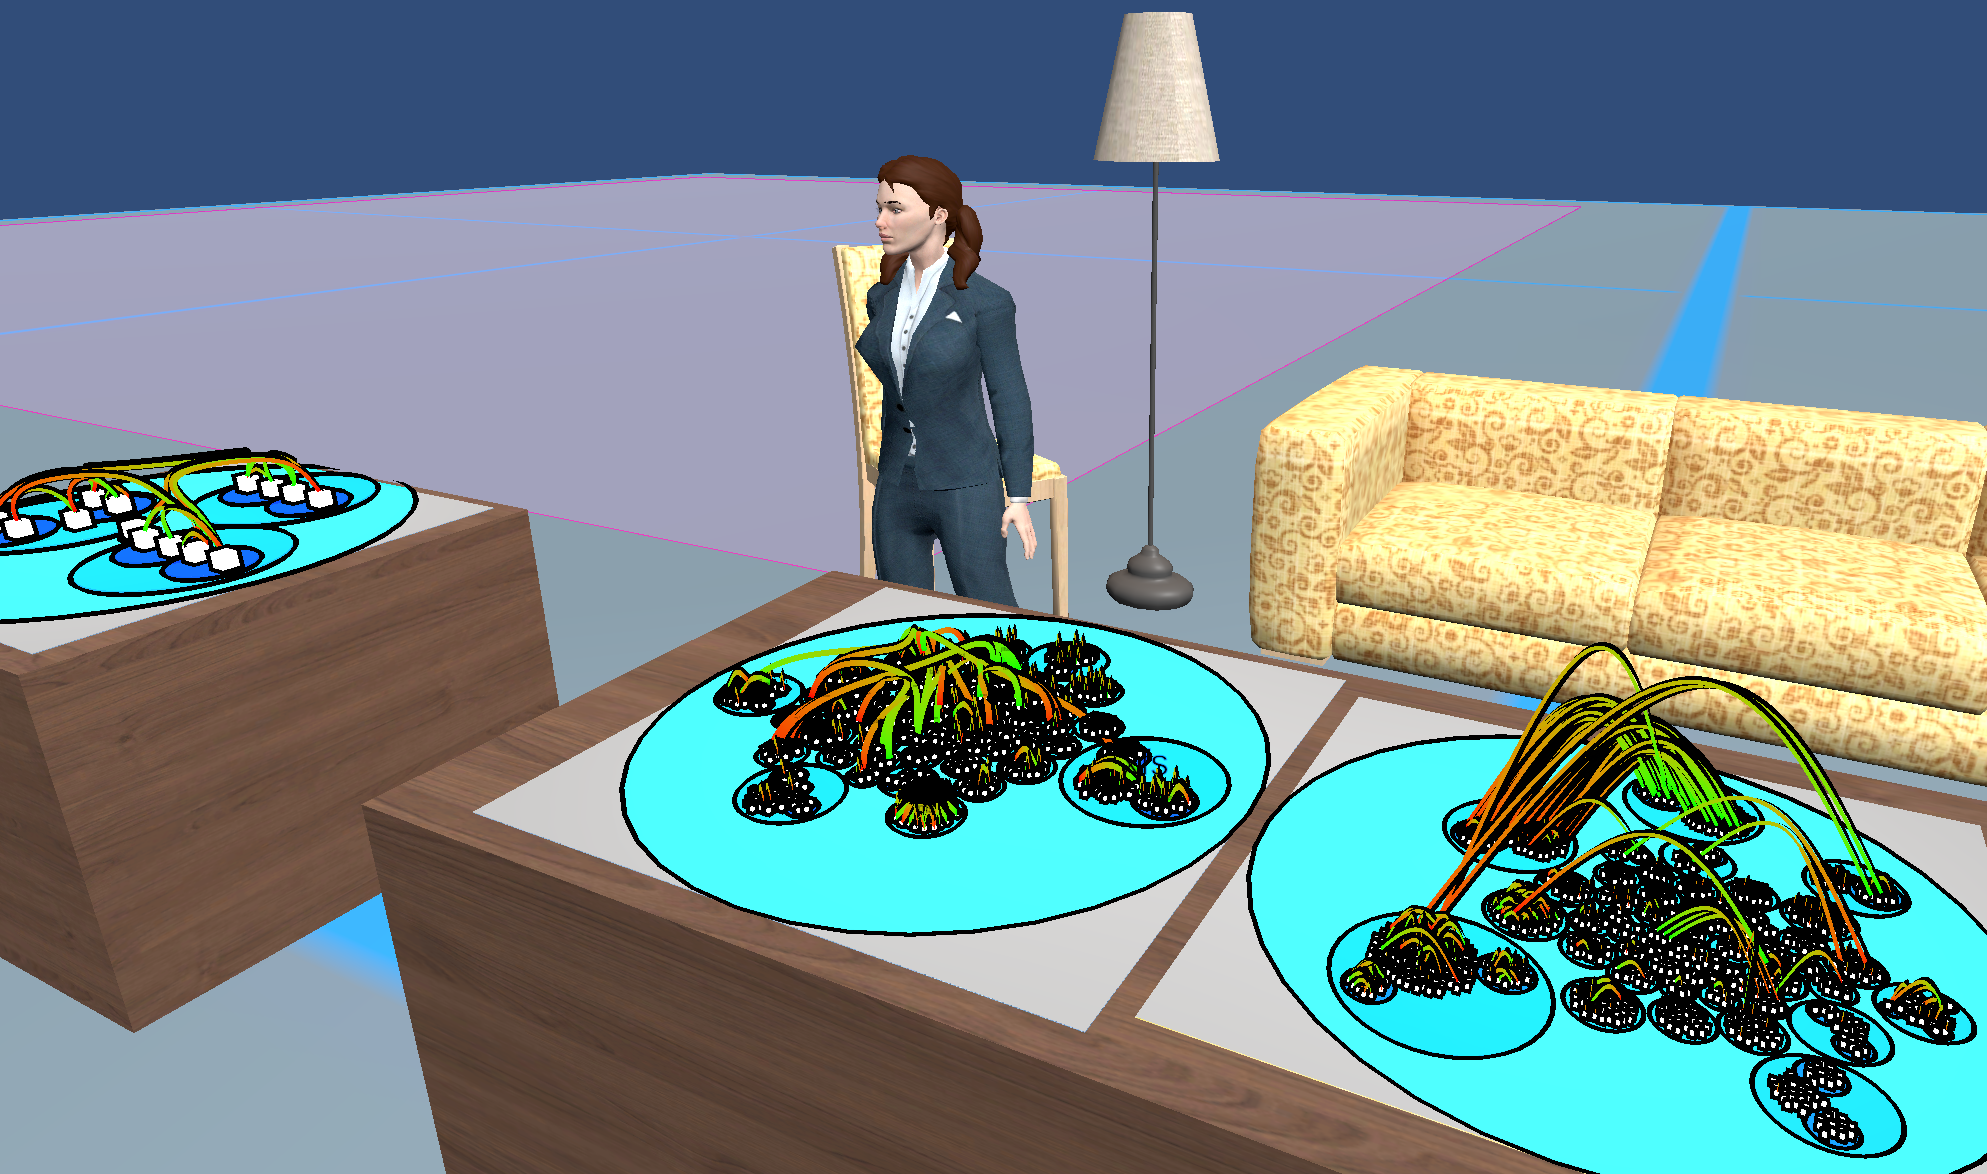
\includegraphics[width=1\textwidth]{Fundamentals/img/SEE.png}
    \caption{An example of \gls{see} used for the user study in chapter \ref{section:evaluation}}
    \label{fig:see_example}
\end{figure}

\subsection{Code Cities}
\label{sec:code_cities}
A \gls{city} is an approach of visualizing software projects.
An example of a \gls{city} by \cite{wettel2007visualizing} can be seen in figure \ref{fig:city_example}.
Since the representation is three-dimensional many metrics can be visualized in a single \gls{city}.
Code Cites could use, as an example, the metrics number of classes as building height, number of attributes as base size and the and the nesting level of a package as the building color (\cite{wettel2008visual}).
The \gls{city} provides an overview of the represented system and by walking around it in \gls{see} the user can get an idea of the structure of the represented system.
On challenge of representing large code bases is the overwhelming amount of information.
Therefore, using metaphors as the \gls{city} aims to avoid overwhelming the user with too much abstract information (\cite{Wettel2008}).
\begin{figure}[htb]
    \centering
    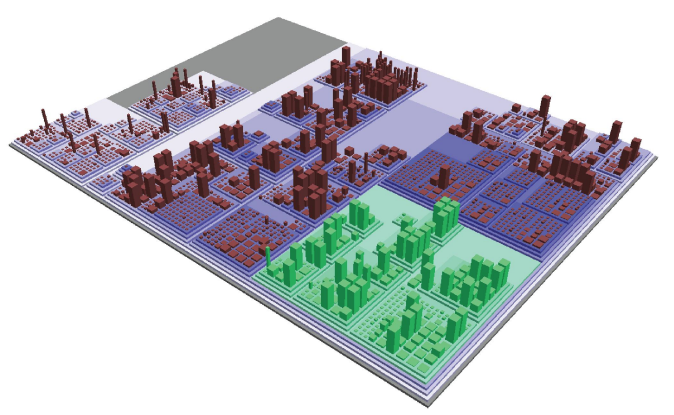
\includegraphics[width=1\textwidth]{Fundamentals/img/code_city.png}
    \caption{An example for a \gls{city} by \cite{wettel2007visualizing}}
    \label{fig:city_example}
\end{figure}

\subsection{Unity}
\gls{unity} is a cross-platform game engine that has been released in June 2005 as \textit{Unity 1.0}.
The engine is not only used for games but also for other industries regarding architecture, automotive or film\footnote{https://unity.com/ (last visited: 22.06.22, 2:39)}.
\gls{unity} started to become successful with its launch in the Apple App Store. 
This is due to the growing popularity of mobile video games and \gls{unity} being on of only few game engines that are optimized for Apple.
The game engine grew ever since and has grown its support for multiplatform development (\cite{nicoll2019unity}).

\subsubsection{Ray Casting}
\label{sec:ray}
Ray casting is basic computer graphics rendering algorithm. 
Rays are cast to determine on their path what can be seen be the camera perspective. 
In the example of figure \ref{fig:ray_example} a local camera coordinate system can be seen.
The lines from the origin on the right are rays that determine the view plane of $z=0$.
\begin{figure}[htb]
    \centering
    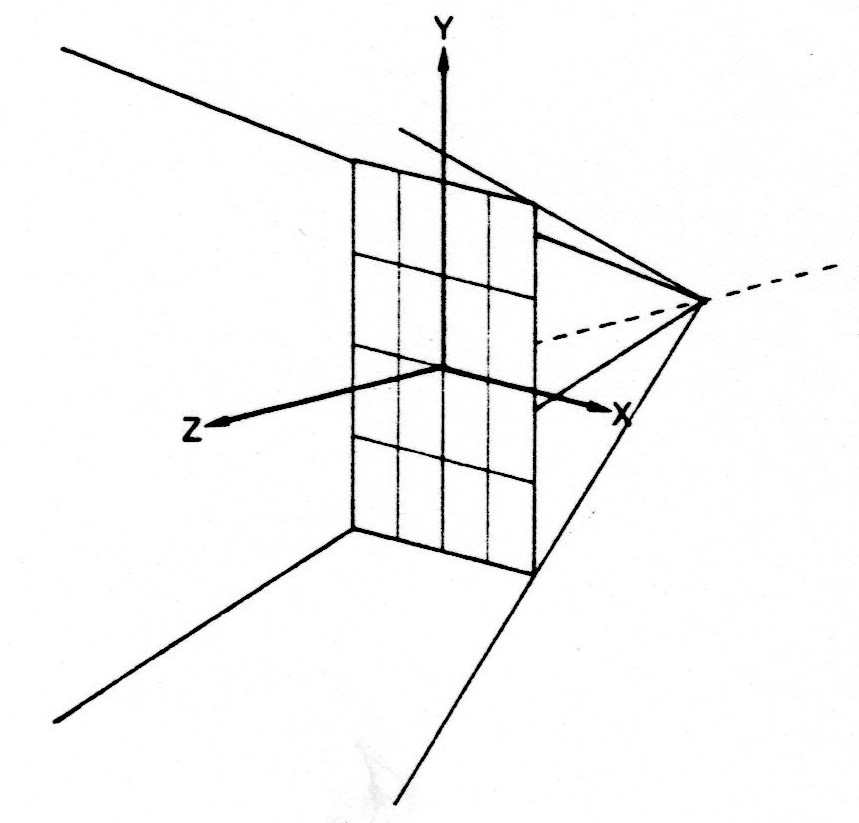
\includegraphics[width=1\textwidth]{Fundamentals/img/ray_casting.jpg}
    \caption{Camera's local coordinate system by \cite{roth1982ray}}
    \label{fig:ray_example}
\end{figure}

Ray casting will also be used to detect the closest object from a certain point on the camera's perspective.
For example objects will often be selected by touch and to determine with object is touched ray casting is needed.
Therefore, a ray will be cast from the center of the touch input and call be the closest object. 
This could also be used to determine if a touch input is on a \gls{city} to allow rotating or moving interactions. 

\subsubsection{Debugging and Testing}
Building another version of a consisting application can take a lot of testing.
Testing in \gls{unity} for \gls{android} applications can be escalated in three steps. 
Debugging always works in combination with the \textit{Microsoft Visual Studio}\footnote{visualstudio.microsoft.com/ (last visited: 24.06.22, 0:12)} debugger, an \gls{ide} for multiple coding languages including \textit{C\#}.

The first and easiest method can be done directly in the \gls{unity} Editor by using the core feature \textit{Play Mode}.
In \textit{Play Mode} the project starts and builds as it would in a final build.
Any changes made in will not be saved and will be reset after leaving \textit{Play Mode}.
However, the building time in the \textit{Play Mode} is much faster than the actual \gls{android} build.
Unfortunately touch input can not be tested on a desktop computer, but the \textit{Play Mode} suffices for testing UIs or other basic changes. 

\begin{figure}[htb]
    \centering
    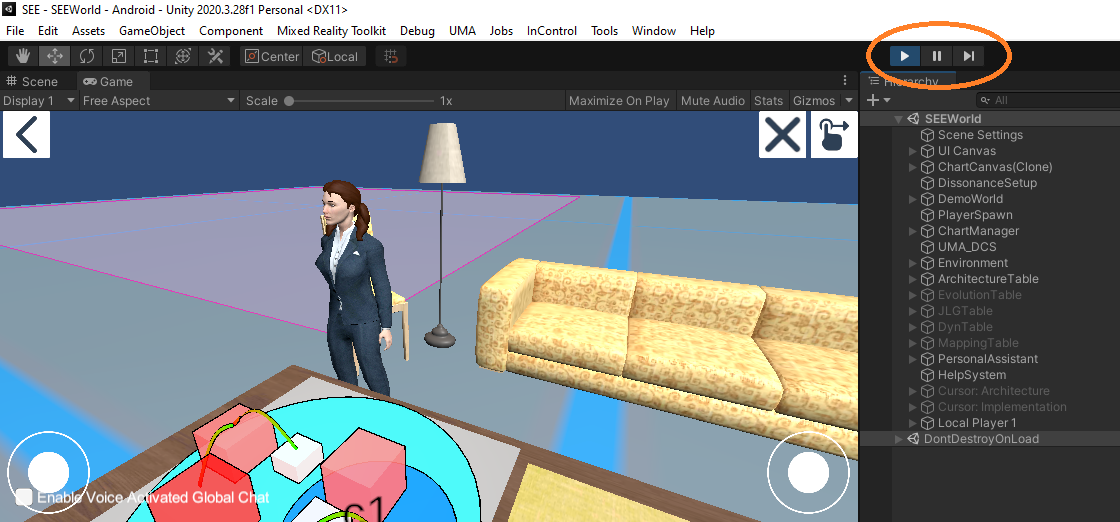
\includegraphics[width=1\textwidth]{Fundamentals/img/play_mode.png}
    \caption{The \textit{Play Mode} can be entered by pressing play at the marked spot}
    \label{fig:play_mode}
\end{figure}

However, if actions with touch input need to be tested, the second method is suitable.
Therefore, \gls{unity} provides the app \textit{Unity Remote}\footnote{https://docs.unity3d.com/Manual/UnityRemote5.html (last visited: 24.06.22, 0:14)}.
The app can be connected via USB with the \gls{unity} Editor.
After hitting the play button the \gls{scene} will also be displayed on the connected device and also take input.
Besides touch input other factors for a mobile application like the accelerometer, gyroscope or the camera can be tested. 
The application however will be build on the desktop computer and not on the \gls{android} device. 

To test the application for example for bugs that cause a crash on some \gls{android} devices the application has to be build and installed on the device.
The device can then be connected with the \gls{ide} via Wi-Fi or USB. 
\gls{unity} also provide an option to let the built application wait for a connection with the \gls{ide}, since the connection can take some time.
This however is more time-consuming than the other to methods. 
An \gls{unity} \gls{android} build can take depending on the project size more than five minutes. 
It should therefore only be a last option and only be used to debug concerns regarding the devices hardware constrains. 

\section{Concept}
\label{section:concept}
In this section a concept of a mobile \gls{see} version will be presented. 
Therefore, a prototype will be created to point out the features that a mobile version of \gls{see} requires.

Prototypes are a common way to express the needs of a system. 
It is a low-cost way of planning an implementation, that can highlight challenges regarding constraints of a system early on.

Even though a prototype will never be able to show every aspect and need of a complex system, it should still help to answering questions like: 
How should the system feel? How should it be implemented, and what are the key features? \cite{houde1997prototypes} 

\gls{see} is meant to be used by multiple platforms such as desktop devices, mobile devices and virtual reality devices.
Each device has different interaction constrains. 
While a desktop user will control the player with mouse and keyboard a mobile user will interact with virtual joysticks on a touchscreen.
Selecting nodes of a \gls{city} will be done by clicking it with a mouse on desktop devices, while a mobile device will require a touch input.

\subsection{Interface}

In the following a paper prototype will be presented that marks out a concept for the mobile interface.
Since the field of mobile development is quite young there few guidelines regarding the design of mobile device interfaces.
A guideline that is widely accepted is problematic to find. \cite{renaud2017demarcating}, \cite{punchoojit2017usability}

Major differences to desktop environments are the screen size, forms of input and input feedback.
To assure as much space is used for the actual interaction of the app the menu should just take as much space as needed.
As a study has found out, a size of at least 8*8 mm is needed to reduce error rates selecting the right button. \cite{conradi2015optimal} \cite{parhi2006target}
TODO WEITER AUSFÜHREN
SHORTCUTS WIE STRG Z NICHT MÖGLICH
 \cite{adipat2005interface} 

Moving the player will be handled with virtual joysticks as seen in figure \ref{fig:joystick}.
The left joystick will move the player through the virtual room and the right will move the camera angle or in other word the direction the player looks at.
The joysticks are placed in the left and right corner and should just take as much space as needed to be handled comfortably.
This way the player is able to navigate through the virtual room with his/her thumps while still having enough space to work on the \gls{city}.

\begin{figure}[htb]
    \centering
    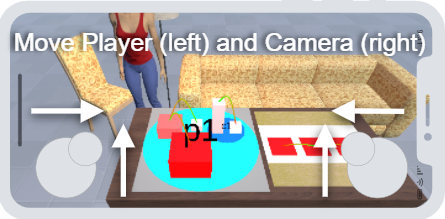
\includegraphics[width=1\textwidth]{Concept/img/joystick.png}
    \caption{Joysticks for moving in \gls{see}}\label{fig:joystick}
\end{figure}

The menu on the top left side seen in figure \ref{fig:quickbar} will be called "quickbar" further on. 
The quickbar can be minimized to safe screen space when not needed. 
The quickbar is designed to offer more general functions that are needed in various situations.
Because there are no shortcuts on mobile devices each function has to have a button to be activated.

The functions are redo and undo which will do an action undone again or revert an action.
Then there is a camera lock that will lock the players perspective to a certain \gls{city} so that the player can only move around the selected city and move closer or further away from it.
The next function is to rerotate a \gls{city}.
That means the \gls{city} that was last rotated will be set back to its initial state of rotation.
Last but not least there will be a button for recentering the city, which will work quite similar to the rerotate button and center the last moved \gls{city}.
The button on the right can be used to collapse or expand the quickbar.
\begin{figure}[htb]
    \centering
    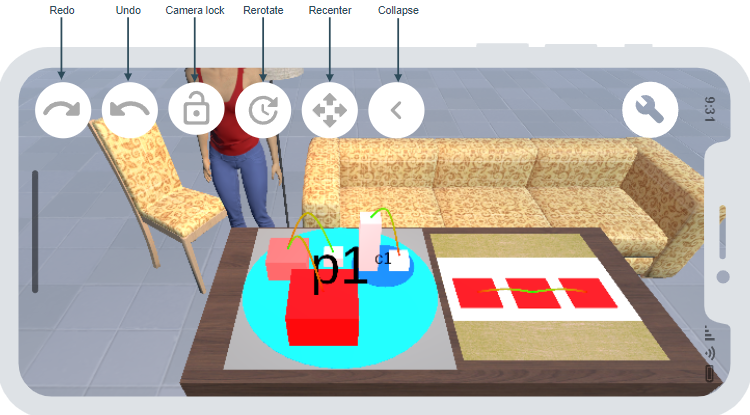
\includegraphics[width=1\textwidth]{Concept/img/quickbar.png}
    \caption{Quickbar for various interactions in \gls{see}}\label{fig:quickbar}
\end{figure}

On the top right side another menu will be placed that contains different interaction modes.
By clicking a button an interaction mode will be selected and moved to the top right corner.
Also, the menu will be collapsed and only the buttons regarding the selected interaction mode shall be shown.
By clicking the button on the top right again the menu shall expand and the other interaction modes shall be selectable.
The other buttons shall be kept in the same order to reduce confusion of the user.

The first interaction mode, seen in figure \ref{fig:select}, is for selecting nodes.
Nodes can be selected by being touched and deselected by being touched again.
There can be multiple nodes selected at once.
The hole selection can be deselected by clicking the deselect button next to the select interaction mode button.
Selected nodes shall be highlighted with a different node color and also display their name.

\begin{figure}[htb]
    \centering
    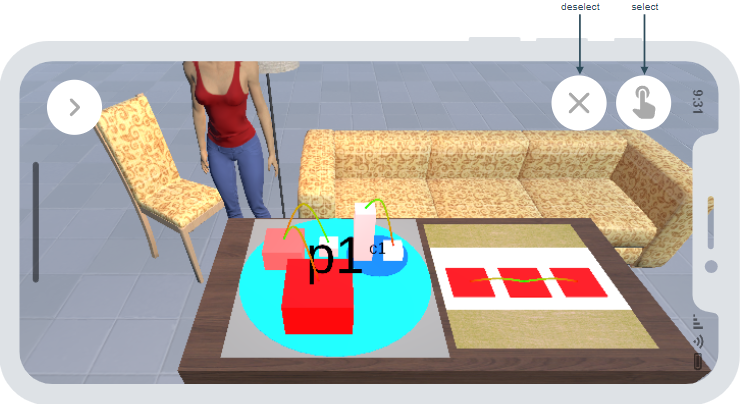
\includegraphics[width=1\textwidth]{Concept/img/menu1.png}
    \caption{Selection mode in \gls{see}}\label{fig:select}
\end{figure}

The second interaction mode, seen in figure \ref{fig:delete}, is for deleting node.
It does not need additional buttons.
Node will be deleted by being touched.-
Unlike in the desktop version there will not be a group deletion interaction because it would require an additional menu panel.
The added functionality would be minimal and selecting a group of nodes, confirming and finally deleting would require a handful more steps and would therefore most likely not be used.

\begin{figure}[htb]
    \centering
    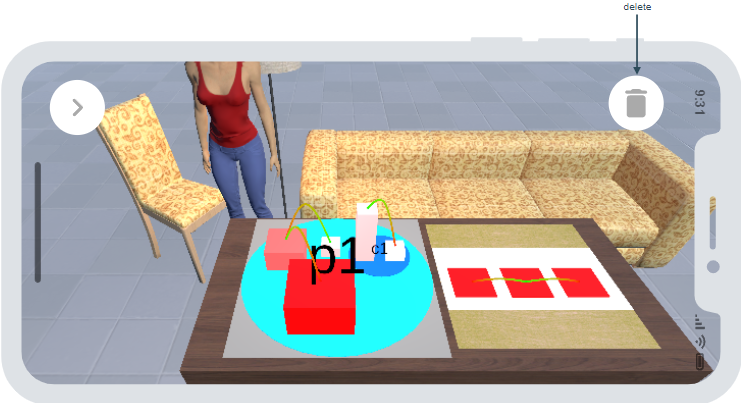
\includegraphics[width=1\textwidth]{Concept/img/menu2.png}
    \caption{Delete mode in \gls{see}}\label{fig:delete}
\end{figure}

The following interaction mode, seen in figure \ref{fig:nodes}, is dedicated to the nodes and edges of a \gls{city}.
Starting on with the "add node" button on the right.
When activated the user can create new node by clicking on a certain spot on the \gls{city} plane. 
The following button on the left is for adding edges.
By selecting two nodes a new edge will be created between them. 
Then, the button one further on the right is for editing nodes.
By touching a node a window will pop up that allows the user to edit the node by changing its name and its type.
Last but not least the button on the left-hand side will be used to scale nodes.
That means the node height and width can be adjusted by first selecting it via touch and then hold a corner and slide it further away from the node center to increase the size or slide it towards the center to decrease the size of the node.
Each button of the node interactions will be marked green after being pressed to indicate that it is active.

\begin{figure}[htb]
    \centering
    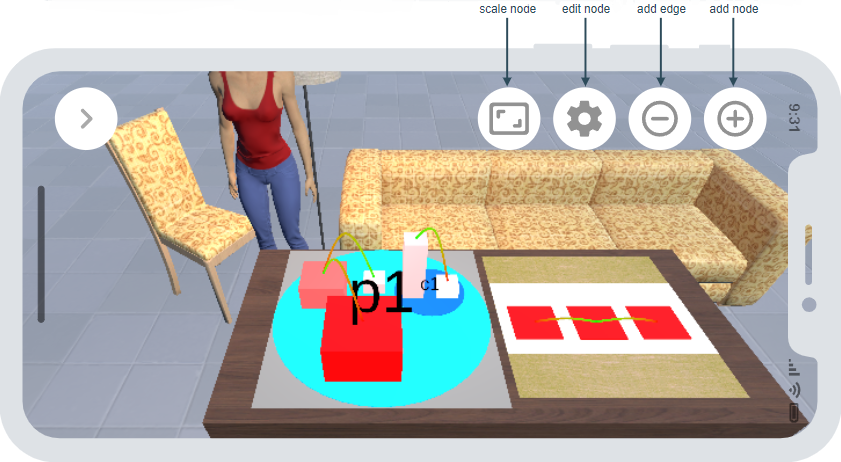
\includegraphics[width=1\textwidth]{Concept/img/menu3.png}
    \caption{Node interactions in \gls{see}}\label{fig:nodes}
\end{figure}

Then there will be a button for rotation interactions that can be seen in figure \ref{fig:rotate}.
Starting with the first activatable button that lets the user rotate the hole \gls{city} by touching any point on it and then sliding away from that point.
Similar to that there will be a button that lets the user rotate just a single node on the \gls{city}.
In addition to that there will be a button that activates the so-called "locked-rotation" mode.
While in "locked-rotation" mode the rotation of a node or \gls{city} will be done in eight predefined steps to a full rotation.
Each step will have the same 45° range.
The last button of this group will be for changing the center of the rotations. 
There are to options: the first option is a center of rotation in the middle of the \gls{city} and the second is in the middle of a node selection made with the interactions seen in figure \ref{fig:select}.
The second option can be activated by pressing the last button.

\begin{figure}[htb]
    \centering
    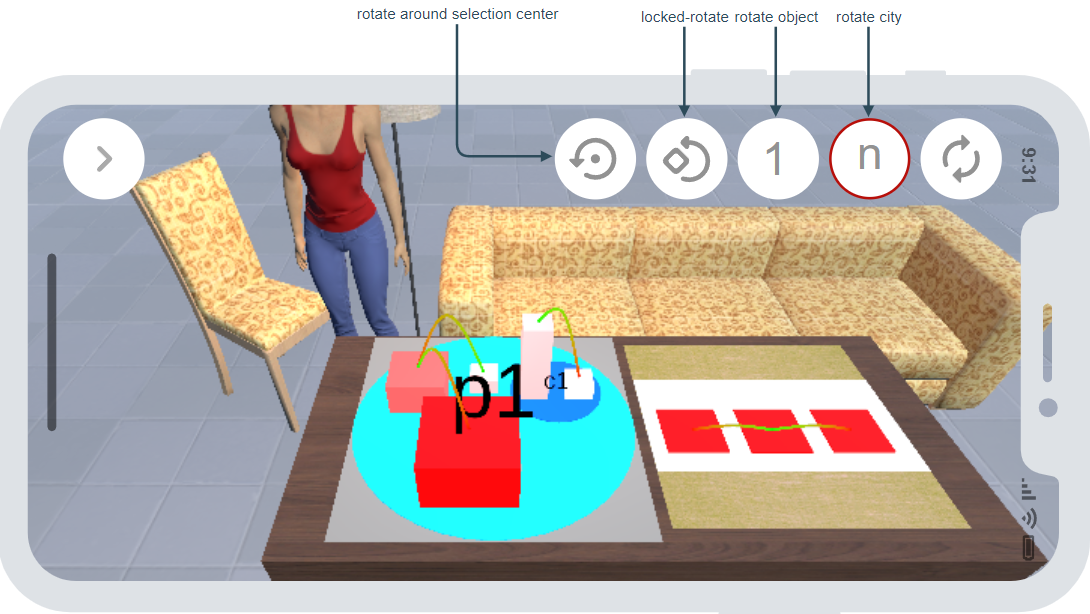
\includegraphics[width=1\textwidth]{Concept/img/menu4.png}
    \caption{Rotation mode in \gls{see}}\label{fig:rotate}
\end{figure}

The last interaction group, seen in figure \ref{fig:move}, is for moving the \gls{city} or a single node.
The move interactions are quite similar to the rotation interactions.
There will be a button to move a hole \gls{city} as well as a button to move only single nodes.
In addition to that there will be a button that restricts the movement of the \gls{city} or node to a predefined direction.
The directions will be again in 45° angles and objects can be moved on a straight line on that angle.
Moving a node or a \gls{city} can be achieved by touching and holding it and then moving it to the desired position.
\begin{figure}[htb]
    \centering
    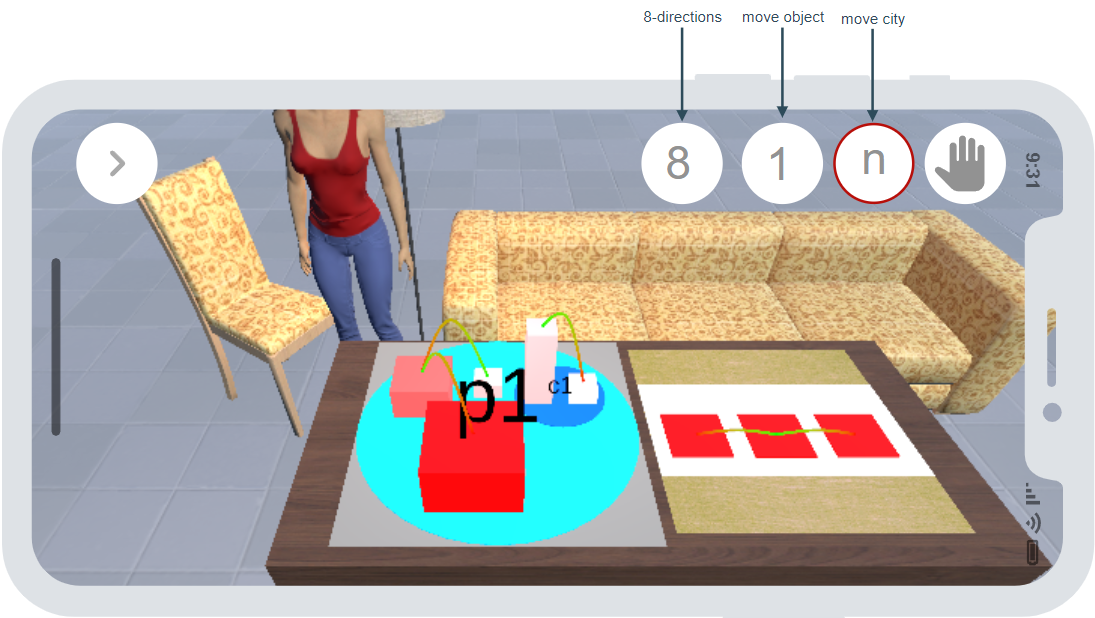
\includegraphics[width=1\textwidth]{Concept/img/menu5.png}
    \caption{Movement mode in \gls{see}}\label{fig:move}
\end{figure}

\subsection{Interaction}

Smartphones are quite limited in space and there are few input possibilities.
Unlike a desktop computer there is no mouse and there is no physical keyboard.
Smartphones use virtual keyboards but due to the restriction of screen space the keyboard is hidden most of the time.
Which would make keyboard shortcuts uncomfortable because the user has to open the keyboard first.
Therefore, smartphones need different ways of interaction such as touch gestures. 

Zooming in to a \gls{city} happens by scrolling on a desktop environment. 
The is no option to scroll on mobile devices, but there are at least two popular alternatives.
The first option would be to double tap on the \gls{city} to zoom in.
The double tap would zoom in, in predefined steps and after reaching a certain level of closeness it would trigger to zoom out again.
In \gls{see} zooming in, in predefined steps might not be precise enough because there could be a quite large \gls{city} or a rather small one.
Finding predefined steps that would fit every situation is rather hard.
Therefore, a second option by zooming in with a two finger gesture might be better. 
In this option the user uses two fingers and slides them towards each other to zoom in or slides the two fingers away from each other to zoom out.
This way there are no predefined steps necessary and zooming interactions can be done precisely.
\subsection{Requirements}
In the following a list of requirements will be given, which will specify in detail what the implementation of a mobile version has to take care of.
The list will be referred to multiple times in the upcoming realization part in chapter \ref{section:implementation}.
Requirements are essential for the planning phase as they give a good fundamental structure for the developer to rely on. \cite{Robertson2012,Stevens2005}
\begin{itemize}
    \item[{[R1]}] The application shall run on Android devices
    \item[{[R2]}] The application shall be controlled via touchscreen
    \begin{itemize}
        \item [{[R2.1]}] The player and camera shall be moved with virtual joysticks
        \item [{[R2.2]}] Needed shortcuts of the desktop version shall be handled with buttons
        \item [{[R2.3]}] Zooming shall be handled with a two finger gesture
    \end{itemize}
    \item[{[R3]}] The user shall be able to select a node of a \gls{city}
    \begin{itemize}
        \item [{[R3.1]}] After selecting the name of the node shall be shown
        \item [{[R3.2]}] The user shall be able to deselect single nodes or a group of nodes
    \end{itemize}
    \item[{[R4]}] The user shall be able to delete nodes
    \item[{[R5]}] The user shall be able to interact with nodes
    \begin{itemize}
        \item [{[R5.1]}] The user shall be able to add nodes
        \item [{[R5.2]}] The user shall be able to add edges
        \item [{[R5.3]}] The user shall be able to edit nodes
        \item [{[R5.4]}] The user shall be able to scale nodes
    \end{itemize}
    \item[{[R6]}] The user shall be able to rotate a \gls{city}
    \begin{itemize}
        \item[{[R6.1]}] The user shall be able to rotate a \gls{city} in 45° steps
        \item[{[R6.2]}] The user shall be able to rotate single objects
        \item[{[R6.3]}] The user shall be able to rotate around a center of selected nodes
        \item[{[R6.4]}] The user shall be able to undo the rotation
    \end{itemize}
    \item[{[R7]}] The user shall be able to move a \gls{city}
    \begin{itemize}
        \item[{[R7.1]}] The user shall be able to move single object of a \gls{city}
        \item[{[R7.2]}] The user shall be able to restore the \gls{city} initial position
        \item[{[R7.3]}] The user shall be able to move a \gls{city} or single node in predefined directions
    \end{itemize}
    \item[{[R8]}] The user shall be able to undo and redo actions
    \item[{[R9]}] The user shall be able to lock the camera to a selected \gls{city}
\end{itemize}
\section{Implementation}
\label{section:implementation}

This chapter will discuss the implementation of the mobile version of \gls{see}.
Starting with the mobile player implementation in section \ref{sec:player}.
Section \ref{sec:player_movement} will give insight on the player movement before section \ref{sec:menu} will discuss the mobile menu.
Next the implemented player action will be introduced in section \ref{sec:player_actions}.
This chapter will close with pointing out the requirements for an \gls{android} build and how they have been handled.
\subsection{Mobile Player}
\label{sec:player}
In this section the mobile player \gls{prefab} will be discussed. 
\gls{see} is supported on multiple platforms and with each platform having different requirements each platform needs to be divided.
Therefore, each platform gets its own player \gls{prefab}.
The mobile player prefab for the \gls{android} version of \gls{see} can be seen in figure \ref{fig:prefab}.

\begin{figure}[htb]
    \centering
    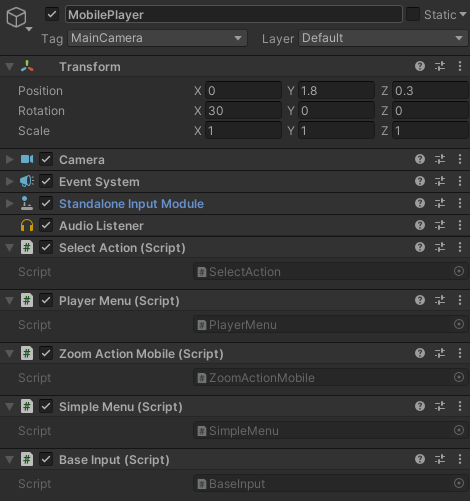
\includegraphics[width=0.8\textwidth]{Implementation/img/mobile_player.png}
    \caption{The mobile player \gls{prefab}}\label{fig:prefab}
\end{figure}

The \gls{prefab} consists of the basic parts provided by \gls{unity} \textit{Camera}, \textit{Event System}, \textit{Standalone Input Module} and \textit{Audio Listener}.
In addition to that the following custom scripts were added.
There is the \textit{SelectAction} and the \textit{ZoomActionMobile} script, which will both be discussed in section \ref{sec:player_actions}, and then there is the \textit{PLayerMenu} script, which creates the right menu based on the player type.
In this case the player type will be \enquote{mobile player} and the menu created (here \textit{SimpleMenu}) will be discussed in section \ref{sec:menu}.

\subsection{Player Movement}
\label{sec:player_movement}
After having creating a player, the player also has to be able to move.
Therefore, the \textit{MobilePlayerMovement} script got added.
The script handles the input by the joysticks seen in figure \ref{fig:joystick}.
To fulfill [R2.1] the player will be moved by using the left joystick and the player's perspective will be handled by the right joystick.

\begin{figure}[htb]
    \centering
    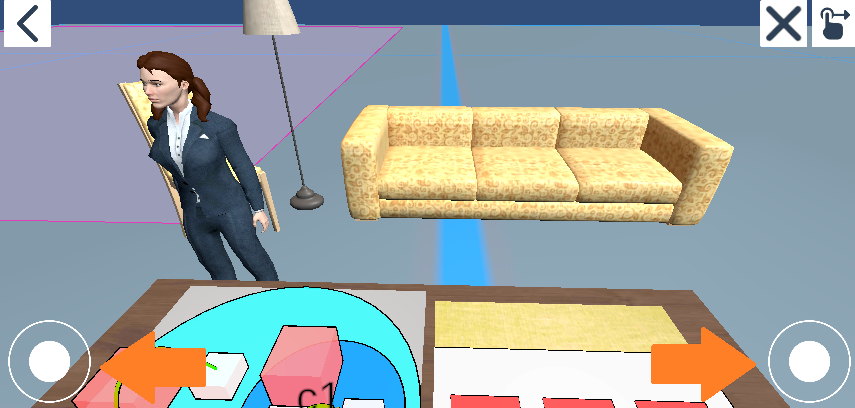
\includegraphics[width=1\textwidth]{Implementation/img/joysticks.png}
    \caption{The joysticks are for moving in the virtual room. The left joystick is for moving the player and the right one is for moving the player's perspective.}\label{fig:joystick}
\end{figure}

For the joystick \glspl{prefab} the \textit{Joystick Pack}\footnote{https://assetstore.unity.com/packages/tools/input-management/joystick-pack-107631\#description (last visited: 17.06.22, 15:21)} \gls{asset} is used.
It contains the design and basic logic for the joysticks.
A joystick returns a horizontal and a vertical value depending on how far the joystick is dragged into a direction.
The left joystick data can then be transformed into player movement as follows:
\begin{enumerate}
    \item Get the horizontal and vertical values from the joysticks
    \item Transform the values into a 3D vector
    \item Combine the values into a velocity vector
    \item Normalize the velocity vector for a smooth transition
    \item Transmit the velocity vector to the player position value
\end{enumerate}

The data of the right joystick shall move the player's perspective, which is implemented as a \gls{unity} camera.
The camera has a pitch angle and a yaw angle as illustrated in figure \ref{fig:camera}.
The angles of the camera will be adjusted with the input from the right joystick. 
For the angles of the player's perspective there is a range from 0° to 360° after reaching an end of this range the value will be transformed to the other end of the range.
In other words if the angle grows higher than 360° it starts at 0° again and if it gets lower than 0° it can go further down from 360°.
That way the player's perspective can move a full rotation.
\begin{figure}[htb]
    \centering
    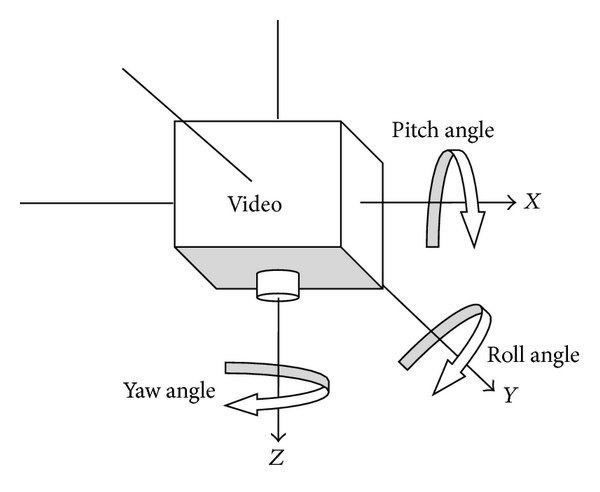
\includegraphics[width=1\textwidth]{Implementation/img/pitch_yaw.jpg}
    \caption{The angles of a camera by \cite{Zhang2014}}\label{fig:camera}
\end{figure}

\subsection{Mobile Menu}
\label{sec:menu}

The mobile menu is essential for the implementation since the input methods of a smartphone in an everyday usage are limited.
The desktop version uses many \glspl{shortcut}, which cannot be used in the mobile version.
These \glspl{shortcut} will replaced with buttons in the menu to fulfill requirement [R2.2].

\begin{figure}[htb]
    \centering
    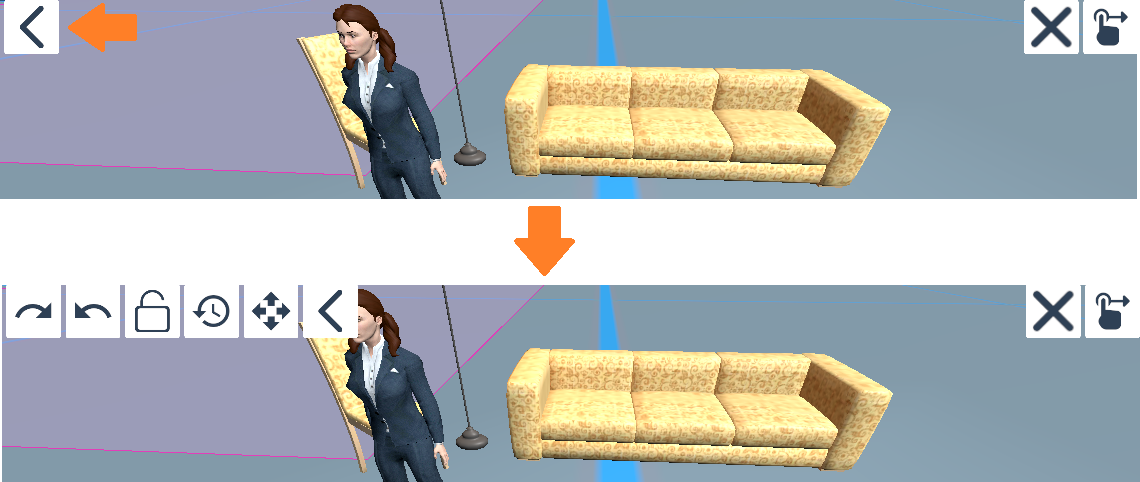
\includegraphics[width=1\textwidth]{Implementation/img/quickmenu.png}
    \caption{The \textit{quickbar} on the left top side of the mobile device. Pressing the button with an orange marked arrow will expand the menu.}\label{fig:quickmenu}
\end{figure}

The menu will be divided into to parts.
The first part, that was named \textit{quickbar} in section \ref{sec:interface}, will be responsible for all interactions that need to be available at all times.
The implemented \textit{quickbar} can be seen in figure \ref{fig:quickmenu}.
By pressing the button on the right end of the \textit{quickbar} the menu can be expanded and minimized to safe screen space when not needed.
The menu also contains buttons for redoing and undoing actions to fulfill requirement [R8].
In addition, that there is a button for a \enquote{locked-mode}.
Unfortunately the button is just a placeholder since the functionality to lock the players view to a city is not available in the desktop version at this time.
Therefore, requirement [R9] can not be completed at the time of this thesis. 

The other part of the menu can be seen in figure \ref{fig:interaction_menu}.
The menu is placed on the right side of the screen, and it contains all the player interactions.
This part of the menu is slightly more complex since the selected button moves to the top, while the other buttons shall remain their initial order.

\begin{figure}[htb]
    \centering
    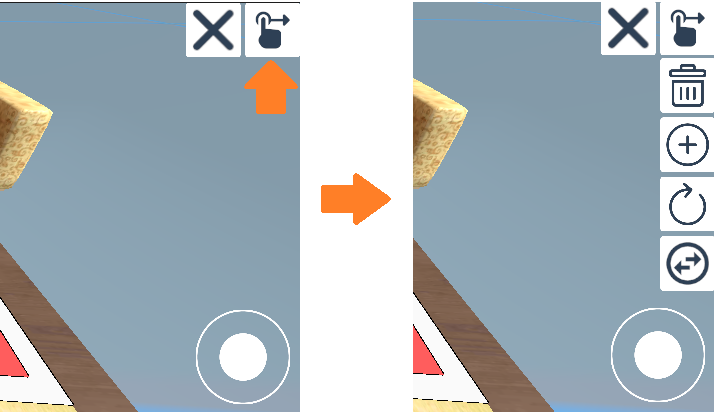
\includegraphics[width=1\textwidth]{Implementation/img/menu.png}
    \caption{The player interaction menu on the right top side of the mobile device. The button on the top right side indicate the active interaction mode. Pressing the same button also expands the menu.}\label{fig:interaction_menu}
\end{figure}

The implementation of the menu on the right is done in the following steps:
\begin{enumerate}
    \item All main buttons get an index
    \item When a button on the far right side gets clicked the index gets saved
    \item The button group with the selected index get shown on the top right side
    \item All other buttons get disabled
    \item By clicking the button on the top right again the other main buttons get reactivated 
    \item The order is as follows: selected index → index in ascending order
\end{enumerate} 
This way the selected interaction mode will always be in the top right corner, while the other buttons remain the same order.

\subsection{Player Actions}
\label{sec:player_actions}

One essential part of the implementation are the player actions. 
Almost all interactions a user can make in \gls{see} differ from the interactions in the desktop version.
In the following the implementation of all mobile player actions will be shortly discussed.

\subsubsection{Zooming}
To fulfill requirement [R2.3] zooming needs to be implemented.
The interaction of zooming in or out of a \gls{city} can be fundamental when working with a large \gls{city} because \glspl{node} become small and especially on a small mobile screen it becomes impossible to interact with those nodes via touch input. 
Therefore, the user has to zoom in to properly interact with the desired node.

Luckily the general zooming function is already implemented in \gls{see}.
The zooming method- requires a center point and a scale of how far the \gls{city} shall be zoomed in or out.
Zooming on a touchscreen will be done by dragging two fingers either towards or away from each other as visualized in figure \ref{fig:zooming}.

\begin{figure}[htb]
    \centering
    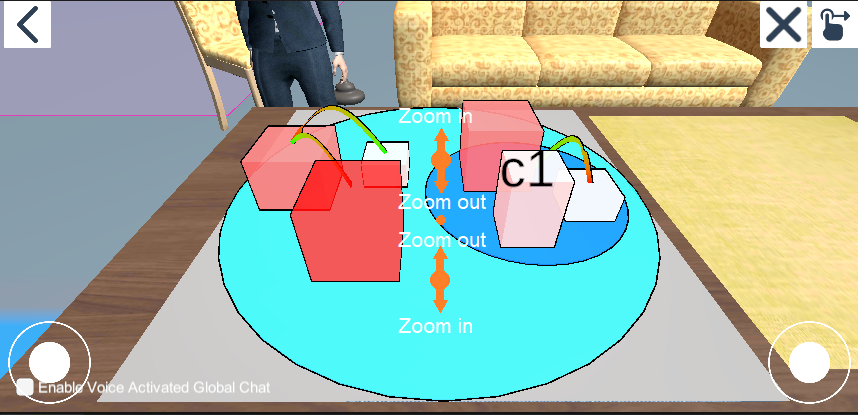
\includegraphics[width=1\textwidth]{Implementation/img/zoom.png}
    \caption{Dragging the two touch points towards each other will zoom out and dragging them away from each other will zoom in.}\label{fig:zooming}
\end{figure}

The implementation of the zooming interaction in done in the following steps: 
\begin{enumerate}
    \item Check if there are two touch inputs on the same \gls{city}. If both inputs are not on the same city zooming is not wanted and will not be activated.
    \item Compute the center of the two touch inputs
    \item Pass the center and dragging range of the two inputs to the zooming function
\end{enumerate}

Note that the direction of zooming has been inverted in the version used for the evaluation in chapter \ref{section:evaluation}.
This is because of the heavy demand by the subjects to invert the direction of zooming since it feel odd.

\subsubsection{Selecting and Deleting}
The interactions of selecting and deleting a \gls{node} or \gls{plane} are quite similar because the user selects or deletes an object by touching it.
The object get determined by a ray cast from the center of the touch position as discussed in section \ref{sec:ray}.

Since the selecting mode is always enabled except when the delete mode is active, the select button really does nothing except ensuring that no other interaction mode is active.
Keeping the selected objects active makes sense for the mobile version because the user cannot hover with a mouse to see the object names.
Therefore, the selection will be kept and not discarded by selecting a different object as in the desktop version.
The deselect button call the already implemented \textit{UnselectAll} method that empties a list of selected items.

To delete interaction works as already mentioned just like in the desktop version. 
The only difference is the type of input. 
Other than in the desktop version the mobile version only supports single deletions and not the deletion of multiple objects at once.
This is due to the limited space for the interactions menu and the results from a multi deletion can also be achieved with the single delete interaction.

The discussed implementation fulfills requirements [R3] and [R4].
\subsubsection{Node Interactions}
The node interactions consist of four types.
The active interaction is always highlighted in green as seen in figure \ref{fig:node}
\begin{figure}[htb]
    \centering
    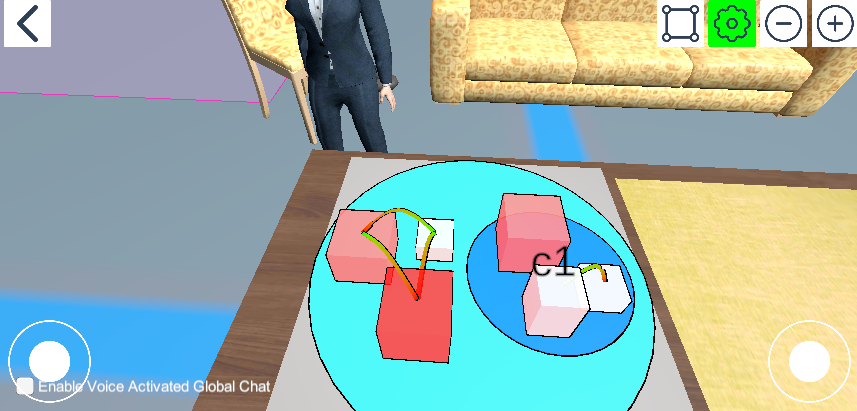
\includegraphics[width=1\textwidth]{Implementation/img/node.png}
    \caption{The node interactions menu. The active node interaction has a green button}\label{fig:node}
\end{figure}

The circled plus button stands for adding a \gls{node}.
Adding \glspl{node} is implemented in the following steps:
\begin{enumerate}
    \item Check if the device is an \gls{android} with a preprocessor tag
    \item Check if there is exactly on touch input
    \item Cast a ray and check if the collided object is of the type \enquote{Node} (\gls{see} does not distinguish between \gls{plane} and \gls{node} as a type)
    \item Create a \gls{node} ad that position with the already implemented \textit{AddChild} method of the class \textit{GameNodeAdder}
\end{enumerate}

The circled minus button is for adding an \gls{edge}.
The implementation is quite similar to the one for adding \glspl{node}.
In this case however the first and second \gls{gameObject} of type \enquote{\gls{node}} will be saved.
After there are two \glspl{gameObject} an \gls{edge} between those objects will be created.

Next in line is the gear button, which can be used for editing \glspl{node}.
The implementation here is almost the same as for the desktop version.
A \gls{node} or a \gls{plane} can be selected by touch and a window will open.
In that window attributes like the name can be changed.
Different from the desktop version is that a virtual keyboard will pop up to let the user type in a new name for example.

Last but not least there is the interaction of scaling a node left.
The implementation here was largely adopted from the desktop version, except again the input type is via touch.
In addition to that the dots that can be selected and dragged are larger in the mobile version (see figure \ref{fig:scale}) because otherwise it would be hard to hit them with a touch input.

\begin{figure}[htb]
    \centering
    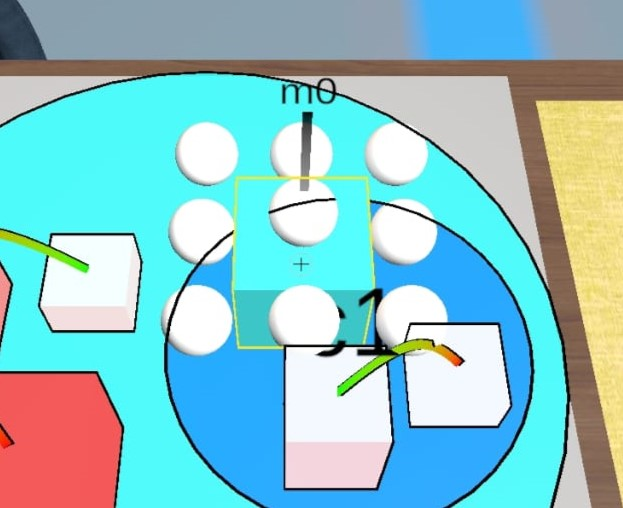
\includegraphics[width=0.7\textwidth]{Implementation/img/scale.jpeg}
    \caption{The node interactions menu. The active node interaction has a green button}\label{fig:scale}
\end{figure}

The listed implementations of the node interactions fulfill the requirements of [R5].

\subsubsection{Rotating}
To fulfil the requirements of [R6] rotating has to be adapted to the mobile version of \gls{see}.
The user can rotate the city either freely or in eight predefined steps.
Figure \ref{fig:rotate} shows a rotation in those eight predefined steps.
As it can be seen the \enquote{8} button is green which means that it is active.
The user can drag from a certain point on the \gls{city} towards a direction the \gls{city} shall be rotated to.

\begin{figure}[htb]
    \centering
    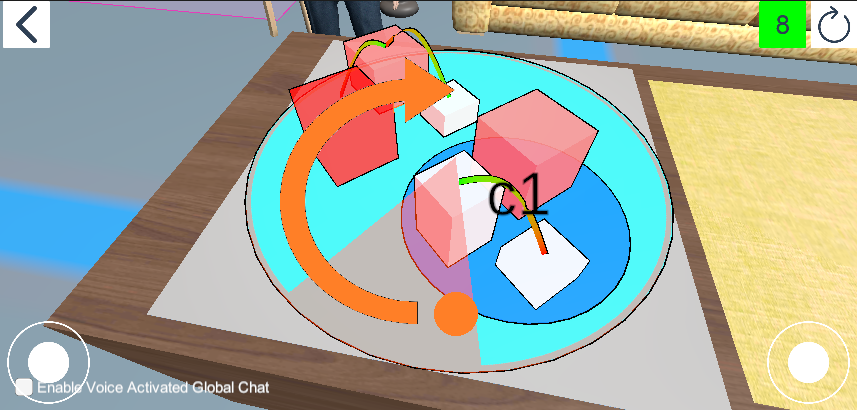
\includegraphics[width=1\textwidth]{Implementation/img/rotate.png}
    \caption{The \gls{city} can be rotated by for example touching the screen on the orange dot and dragging from there like the arrow indicates.}\label{fig:rotate}
\end{figure}

The implementation for the interaction of rotating is done in the following steps:
\begin{enumerate}
    \item Check if there is exactly one touch input on an object of the type \enquote{\gls{node}}.
    \item Check if the \enquote{8} button is active
    \item Calculate the new position of the \gls{city} just like in the desktop version of \gls{see}
\end{enumerate}
\subsubsection{Moving}
Last but not least the player action of moving a \gls{city} or object has to be implemented to fulfill the requirements of [R7].
The user can touch a certain point on a \gls{city} and drag it to move it as visualized in figure \ref{fig:move}.
The same can be done with any \gls{node} or \gls{plane} by activating the \enquote{1} button.
Same as for the rotate-interaction the user can also activate the \enquote{8} to move an object or city in one of eight predefined directions.
Also, by selecting the \enquote{1} or \enquote{8} button it will turn green to indicate that it is active.

\begin{figure}[htb]
    \centering
    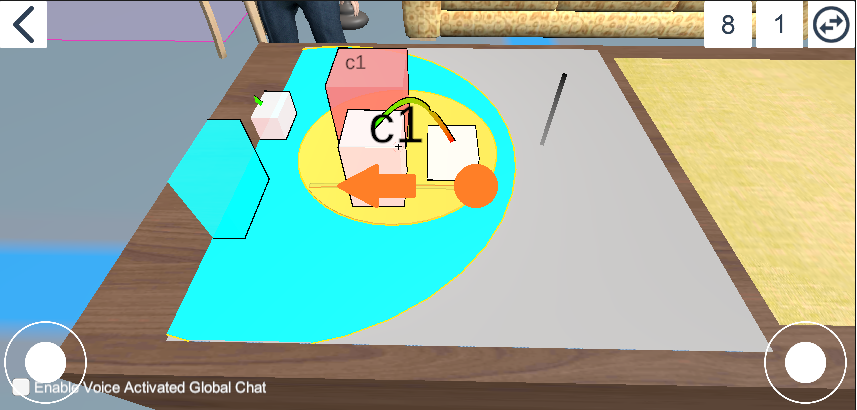
\includegraphics[width=1\textwidth]{Implementation/img/move.png}
    \caption{The \gls{city} can be moved by touching and dragging it to a desired direction.}\label{fig:left}
\end{figure}

The implementation is done similar to the one for the rotate-interaction. 
The only thing added here is the check whether the \enquote{1} button is active or not.

Not that for the rotate and move interactions the \enquote{n} buttons have been removed (see figure \ref{fig:rotate_proto} and figure \ref{fig:move}).
This is because these buttons are not needed since the initial mode when entering the interaction is already for the hole \gls{city}.
Also, the rotate object button and the rotate around selection center button have been removed. 
Rotating around a selection center will always be activated and can be deactivated by removing the selection of objects.
Rotating single objects is not intended as an interaction in \gls{see}.

\subsection{Android Build Requirements}
The last part of this chapter will discuss the requirements to build a version of \gls{see} on \gls{android} to fulfill the last requirement [R1].
In the following there will be a deeper look at the challenges porting \gls{see} to android devices brings. 


\subsubsection{Conditional Compilation}

\gls{see} uses as it is usual for a medium to large \gls{unity} project many \glspl{asset}.
Unfortunately not all \glspl{asset} support a \gls{android} implementation.
Therefore, the unsupported assets have to exchanged or excluded from the implementation.
Some unsupported \glspl{asset} are \textit{Valve} and \textit{UnityEngine.Windows.Speech}.
The \textit{Valve} \gls{asset} is required for the \gls{vr} implementation of \gls{see} and \textit{UnityEngine.Windows.Speech} is fundamental for the speech assistant \enquote{See}.
Since the \glspl{asset} are not supported but still needed in the project they need to be excluded. 

Unity offers a way to compile only partial code. 
Therefore, it uses the \textit{directives}\footnote{https://docs.unity3d.com/Manual/PlatformDependentCompilation.html (last visited: 21.06.2022, 1:27)} of the C\# language. 
These the hash character (\#) followed by \textit{if} or \textit{endif} to mark code areas with a condition.
\gls{unity} has platform scripting symbols like \textit{UNITY\_ANDROID} to set conditions for code areas to be compiled for a certain device or not.
The following code example shows how the technique is used in this project. 

\begin{minipage}{\linewidth}

\begin{lstlisting}[language=C]
using SupportedPackage
#if not UNITY_ANDROID
using NotSupportedForAndroidPackage
#endif 

    SomeClass
    {
    ...
    SomeSupportedPackageMethod()
    ...
    #if not UNITY_ANDROID
    SomeNotAvailableMethodForAndroid()
    #endif
    ...
    }
\end{lstlisting}

\end{minipage}

Examples like this can be found many times in the \gls{see} project. 
In addition to that there are some cases where the main code is exchanged whether the device is an \gls{android} or not.
For example the player actions discussed earlier in this chapter require touch input and can not use the hover effect of a mouse cursor on a mobile device.
Therefore, on mobile devices the touch input code will be used and on desktop devices the mouse hover code, but both code parts use the same methods and variables.
Having two separated classes would make up redundant code. 
On the other hand side excessive use of conditional compilation makes it harder to maintain code because it might have to be adjusted at multiple points for a single change.
This way part of the code could easily be forgotten and lead to bugs.

\subsubsection{File Loading}
One last challenge for the mobile implementation of \gls{see} was how files are handled in the project.
\gls{see} uses specify file space for \gls{unity} called \textit{StreamingAssets}\footnote{https://docs.unity3d.com/Manual/StreamingAssets.html (last visited: 21.06.22, 2:47)} to store for example the various states of an Evolution-\gls{city}.
An Evolution\gls{city} visualizes multiple states of development.
Only the first state is preloaded the other states are stored in the \textit{StreamingAssets} and are loaded at runtime. 
The problem however is that an \gls{android} application is packed into an \gls{jar}.
Files inside a \gls{jar} cannot be obtained without further ado.
To achieve access to files that are not initially loaded \textit{WebRequests}\footnote{https://docs.unity3d.com/ScriptReference/Networking.UnityWebRequest.html (last visited: 21.06.22, 3:13)} have to be used for an \gls{android} implementation. 
Therefore, once again the code needs to be divided and handled with conditional compilation.
This has to be done at every point in the code where files are obtained the common way with \textit{SystemIO} methods. 


\subsubsection{Restructuring}
\label{sec:restructure}
The disadvantage of conditional compilation is that it makes code harder to maintain as discussed earlier.
To minimize this disadvantage it was thought of restructuring the entire project to only have conditional compilation at a core component of \gls{see}.

The concept idea was to restructure the project in a way that from a core component all the different versions get initialized and only in that core component conditional compilation gets used.
All components would have abstract super classes that could be easily supplemented with assets that are not available for all platform.
The platform specific classes would then only be compiled for a certain platform build, since they are divided in the core class.

Unfortunately \gls{see} is already entangled and a restructuring in the described way above would take a high effort.
\gls{see} already has many components that depend on other part of \gls{see}. 
These parts however depend also on other parts of \gls{see}. 
Restructuring and setting a new order for the parts of see that support the idea of a core part of \gls{see} would take too much effort for this thesis and was therefore not implemented.
\section{Evaluation}
\label{section:evaluation}
In the following chapter the mobile implication of \gls{see} will be evaluated in a user study.
Therefore, the mobile application will be compared with the desktop version.

This chapter will start with a description of the desktop version and its main differences in section \ref{desktop}.
Further on, a defined aim and precise hypotheses for the user study will be explained in section \ref{aim}.
After sketching the first experiment set up in section \ref{experiment}, the actual experiment set up will be discussed in detail in section \ref{real} including the used survey tool, questionnaires and the pilot study.
This chapter will then be closed by discussing the results of the user study in section \ref{results} and talking about the threats of validity in section \ref{sec:validity}.
\subsection{SEE Desktop}
\label{desktop}
In this section the desktop version of \gls{see} will be explained.
In this evaluation the mobile version of \gls{see} will be compared with the desktop version.
Therefore, it is necessary to take a deeper look at the differences between those two versions.
Especially at how the interactions differ and what impact it could have on the user experience.

One outstanding difference from the desktop version to the mobile version is the selection of the interaction modes.
While in the mobile version the menu for the interaction modes is always visible, in the desktop version a menu screen opens by pressing space as seen in figure \ref{fig:menu}.
Alternatively interaction modes can be changed by pressing one of the "1-9" keys, which however requires the user to memorize which number belongs to which mode.

\begin{figure}[htb]
  \centering
  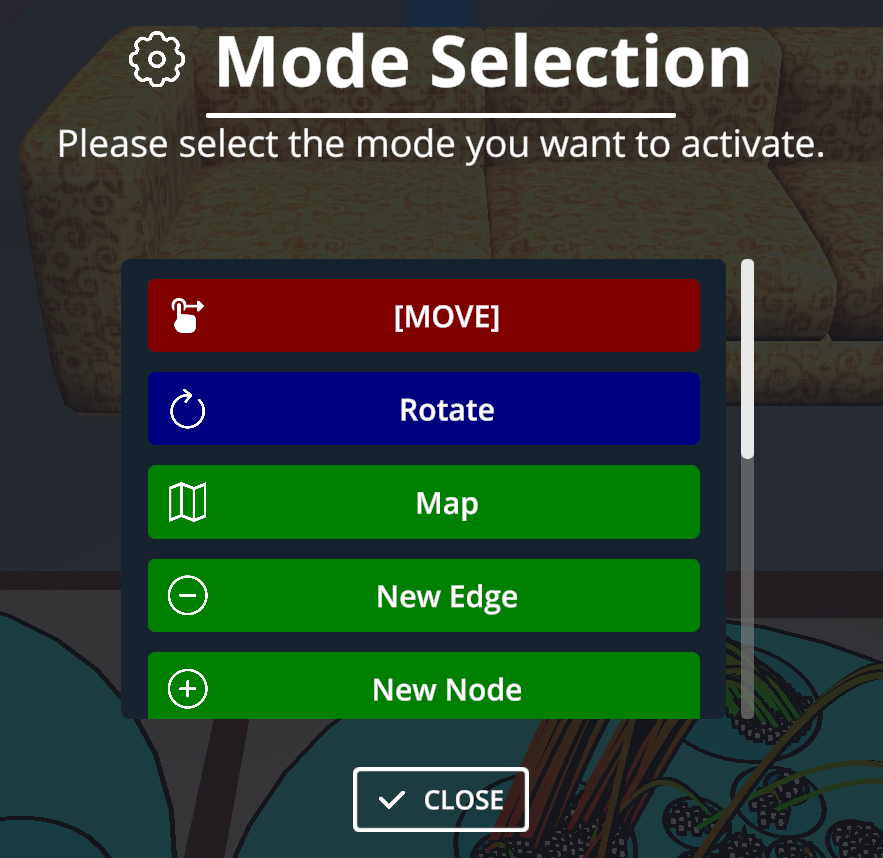
\includegraphics[width=0.8\textwidth]{Evaluation/img/menu.png}
  \caption{The desktop menu for selecting interaction modes.}\label{fig:menu}
\end{figure}

Another difference is the type of user input.
The desktop version uses mouse hovering to display the name of a hovered \gls{node} or \gls{plane}.
This is a faster method than touching the object first in the mobile version.
In addition to that, in the mobile version the object also has to be deselected otherwise there will be a lot of \gls{node} and \gls{plane} names displayed, and it will soon get quite messy.
Also, the precision of object selection differs because touch input can never be as precise as selecting with a mouse cursor.
This could force the mobile user to zoom further in because with a touch input it will not be possible to select small objects like it might be with a cursor.
This, of course, would require more time.

One more key difference is the available keyboard for desktop users.
It allows using \glspl{shortcut}, which make some menu items unnecessary but also requires the user to memorize those \glspl{shortcut}.
The desktop version for example uses the "R" key in the move and rotation mode to recenter or rerotate a \gls{city}.
In the mobile version in opposition, the user will find a button for both actions.
With the right amount of training, both actions should probably equal in the amount of time they need but the mobile version sacrifices screen space for those buttons.
If however the user has to type more text like in renaming objects, the common desktop keyboard should come in handy, as a study from \cite{kim2014differences} shows that even at a same keyboard size, a virtual one will lack in productivity.
\subsection{Aim and Hypothesis}
\label{aim}
The aim of this user study is to answer the research question discussed in section \ref{research}.
In order of answering the research question, the finished prototype of the mobile extension shall be evaluated.
Therefore, the system shall be compared on \gls{android} smartphones as well as desktop computers.
Comparing these two use cases shall give insight on how much impact the constraints of mobile devices have on the \gls{usability} and overall user experience.
To measure the difference between the desktop and the mobile version, the following hypotheses will be used.
The two aspects \textit{Performance} and \textit{\gls{usability}} will be measured in the following study and each aspect will have a null hypothesis and an alternative hypothesis.
\begin{enumerate}[{label=\alph*)}]
  \item \textbf{Performance:} The time required for a task in \gls{see} desktop will be called $t_D$ and for mobile $t_M$.
        \begin{itemize}
          \item \textit{Null Hypothesis} $H_{a0}$: The time required in \gls{see} desktop is higher or the same as the time required in \gls{see} mobile: $t_M \geq t_D$
          \item \textit{Alternative Hypothesis} $H_{a1}$: The time required in {\gls{see}} desktop is lower than the time required in \gls{see} mobile: $t_D < t_M$
        \end{itemize}
  \item \textbf{Usability:} Two aspects are measured for \gls{usability}. First the \gls{ASQ}-Score as a \gls{post-task} result and second the \gls{sus}-Score as a \gls{post-study} result.
        \begin{enumerate}[label=\roman*)]
          \item \textbf{ASQ:} Once again the aspect has to be split into three sub-aspects, because the three questions of the \gls{ASQ} are independent:
                \begin{enumerate}[{label=\arabic*)}]
                  \item The \gls{ASQ}-Score for \textit{complexity} for \gls{see} desktop is called $A_{cD}$ and for \gls{see} mobile is called $A_{cM}$
                        \begin{itemize}
                          \item \textit{Null Hypothesis} $H_{b0}$: The \gls{ASQ}-Score for \textit{complexity} is higher or even for \gls{see} mobile than on \gls{see} desktop: $A_{cM} \geq A_{cD}$
                          \item \textit{Alternative Hypothesis} $H_{b1}$: The \gls{ASQ}-Score for \textit{complexity} is higher for \gls{see} desktop than on \gls{see} mobile: $A_{cD} > A_{cM}$
                        \end{itemize}
                  \item The \gls{ASQ}-Score for \textit{effort} for \gls{see} desktop is called $A_{eD}$ and for \gls{see} mobile is called $A_{eM}$
                        \begin{itemize}
                          \item \textit{Null Hypothesis} $H_{b0}$: The \gls{ASQ}-Score for \textit{effort} is higher or even for \gls{see} mobile than on \gls{see} desktop: $A_{eM} \geq A_{eD}$
                          \item \textit{Alternative Hypothesis} $H_{b1}$: The \gls{ASQ}-Score for \textit{effort} is higher for \gls{see} desktop than on \gls{see} mobile: $A_{eD} > A_{eM}$
                        \end{itemize}
                  \item The \gls{ASQ}-Score for \textit{information} for \gls{see} desktop is called $A_{iD}$ and for \gls{see} mobile is called $A_{iM}$
                        \begin{itemize}
                          \item \textit{Null Hypothesis} $H_{b0}$: The \gls{ASQ}-Score for \textit{information} is higher or even for \gls{see} mobile than on \gls{see} desktop: $A_{iM} \geq A_{iD}$
                          \item \textit{Alternative Hypothesis} $H_{b1}$: The \gls{ASQ}-Score for \textit{information} is higher for \gls{see} desktop than on \gls{see} mobile: $A_{iD} > A_{iM}$
                        \end{itemize}
                \end{enumerate}

          \item \textbf{SUS:} The \gls{sus}-Score is called $S_D$ for \gls{see} desktop and $S_M$ for \gls{see} mobile.
                \begin{itemize}
                  \item \textit{Null Hypothesis} $H_{e0}$: The \gls{sus}-Score is higher or even for \gls{see} mobile as for \gls{see} desktop: $S_M \geq S_D$
                  \item \textit{Alternative Hypothesis} $H_{e1}$: The \gls{sus}-Score is lower for \gls{see} mobile than for \gls{see} desktop: $S_M > S_D$
                \end{itemize}
        \end{enumerate}
\end{enumerate}

The experiment will be participated by different groups:
\begin{enumerate}
  \item \textbf{\gls{see}-developer:} They are already experienced with \gls{see}-desktop.
        They are also experienced with software development and with first person games because they tried at least \gls{see} itself, which counts as first person game experience.
  \item \textbf{Non-\gls{see}-developer:} This group has to be divided into four subgroups as follows:
        \begin{itemize}
          \item \textbf{Software development and third person game experience:} They are more likely to understand the \gls{city} metaphor and are also more likely to be comfortable with the controls in \gls{see}.
          \item \textbf{Software development experience:} They are more likely to understand the \gls{city} metaphor and therefore might be able to find \glspl{node} faster.
          \item \textbf{First person game experience:} They are also more likely to be comfortable with the controls in \gls{see}.
          \item \textbf{No experience:} They do not benefit from experience and therefore have to learn the most to interact in \gls{see}
        \end{itemize}
\end{enumerate}

After the experiment the two versions of \gls{see} can be compared as well as all above listed groups. 
This should give a detailed answer to the research question of this thesis.
\subsection{Experiment Set Up}
\label{experiment}
The system shall be tested in two groups, each starting with a different device.
Each group does the test on both devices, but one group will start with the mobile application and the other one with the desktop application.
The participants will be randomly assigned to the groups.
The subjects will get various tasks to test the \gls{usability} of the two applications.
Afterward, the users will get a survey in English to document their impressions.
\begin{figure}[H]
  \centering
  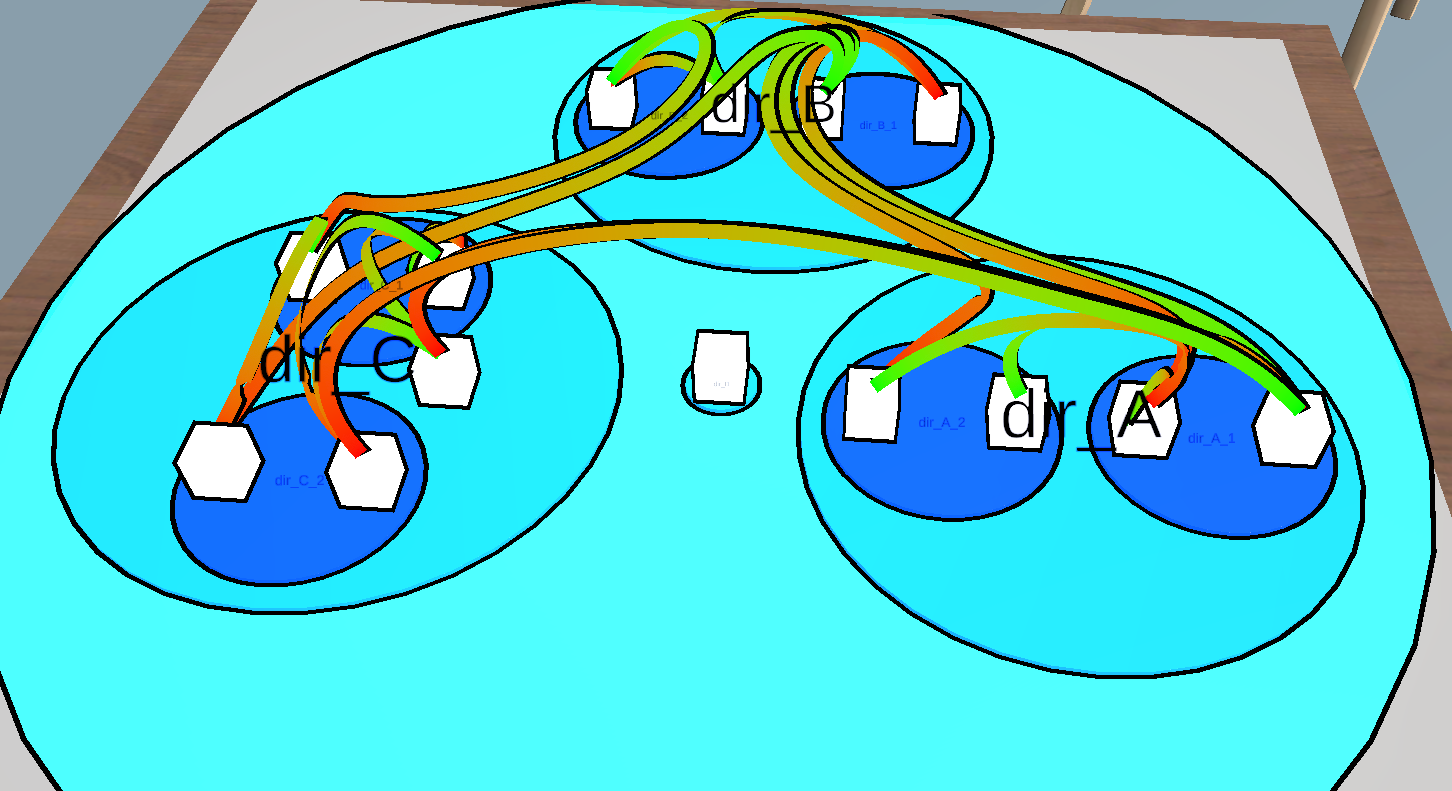
\includegraphics[width=1\textwidth]{Evaluation/img/city_1.png}
  \caption{The first \gls{city} for the user study}\label{fig:city1}
\end{figure}

\begin{figure}[H]
  \centering
  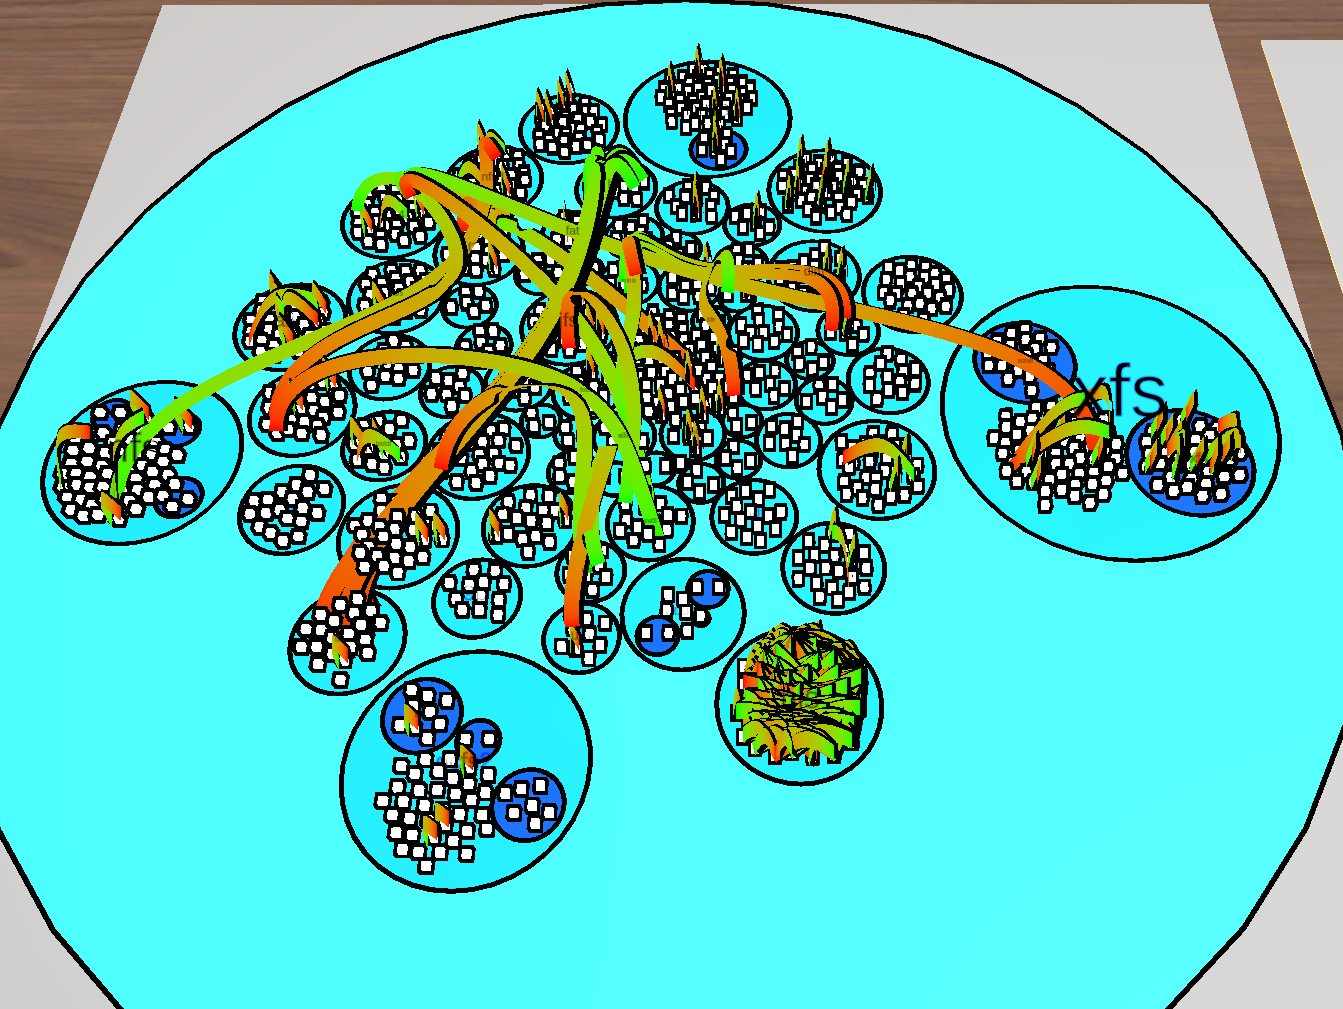
\includegraphics[width=1\textwidth]{Evaluation/img/city_2.png}
  \caption{The second \gls{city} for the user study}\label{fig:city2}
\end{figure}

\begin{figure}[htb]
  \centering
  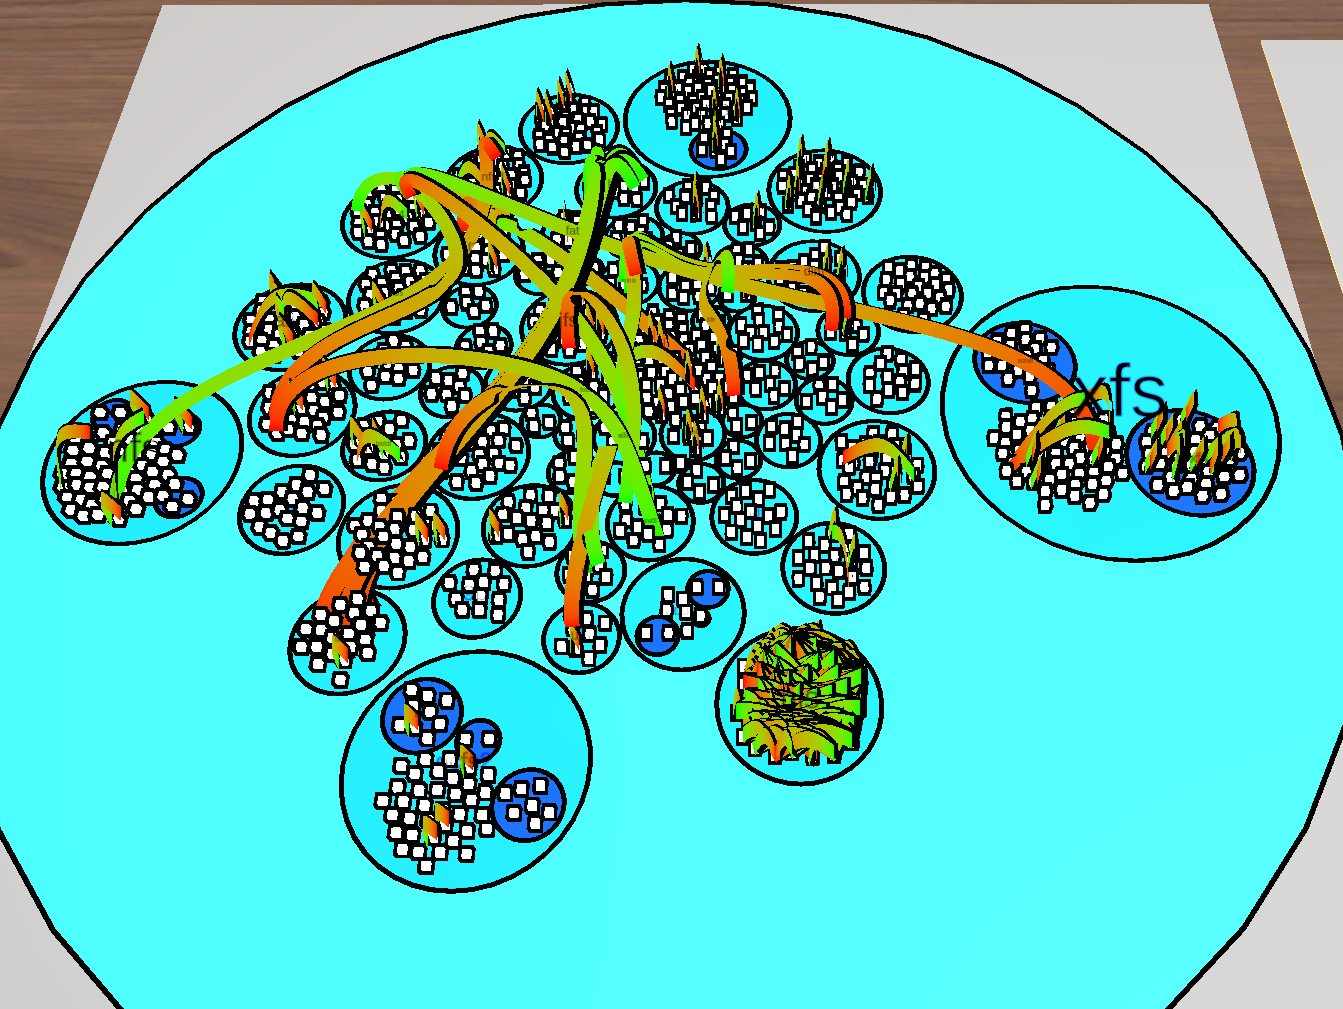
\includegraphics[width=1\textwidth]{Evaluation/img/city_3.png}
  \caption{The third \gls{city} for the user study}\label{fig:city3}
\end{figure}
In this survey the subjects will be asked various demographic questions as well as what \gls{android} device and version they will be using.
In addition to that, the subjects will be asked if they are experienced with \gls{see} and if they are experienced with software development.
Before the subjects will be asked to solve various tasks, they will be asked to watch a short tutorial video on each application.
After the video, they will get a training task where every subject can get used to the system and ask questions if they have trouble solving the training task or using \gls{see} in general.
The overseer will also make sure that every essential action will be practiced such as zooming and moving the \gls{city}.
Figure \ref{fig:city1} shows a small arranged \gls{city} that shall be used for the training tasks.
The structure of the training \gls{city} is generic and follows a simple pattern.
This shall ensure that the user can focus on the training and that the user does not get overwhelmed.

Following the first questions and the training, the subjects can start with the main tasks.
For each application there will be two tasks and after each task the subjects will be handed a \gls{post-task} questionnaire.
Last but not least, there will be another questionnaire that aims to scale the \gls{usability} of the two applications.
For the \gls{post-task} questions the \gls{ASQ} will be used and for the \gls{usability} questions \gls{sus} will be used.
Both questionnaires will be discussed later on in section \ref{questionaires}.
For each main task the overseer will also take the completion time of every main task.
The first and second task on the first device will be performed on the \gls{city} that can be seen in figure \ref{fig:city2} and the third and forth task on device two will be performed on the \gls{city} that can be seen on figure \ref{fig:city3}.
These examples are much larger than the training \gls{city} and represent real life code.
The second \gls{city} shows the file system of Linux and the third one shows the network component of Linux.
That way the tasks might reflect better on real world uses for \gls{see}.

To not exhaust the testers too much the experiment shall not take longer than one hour.
This also ensures that there is no to little variance due to exhaustion.
Each participant might have a different concentration span, but this shall not be the focus of this experiment.

\subsection{Realization}
\label{real}
The following sections will cover the realization of the previously planned study. 
The choice of the used survey tool and questionnaires will be explained in section \ref{survey} and section \ref{questionaires}.
Afterward, a pilot study will be executed to test the study and possibly find missing aspects in section \ref{pilot}.
Finally, the final experiment set up will be discussed in section \ref{final}.

\subsubsection{Survey Tool}
\label{survey}
As a survey tool Google Forms\footnote{https://www.google.com/forms/about/ (last visit: 05.06.2022)} will be used.
The survey tool has to fulfill the following requirements: 
\begin{itemize}
  \item The study will be online because an overseer has to attend every experiment, and therefore it comes in handy to be flexible in terms of location. For this reason the survey shall be fully in a browser. 
  \item The survey tool should be free to use.
  \item Subjects shall be anonymous.
  \item The results shall be exportable in a data format like \gls{csv}.
  \item Subjects should have the option to presave their answers. In addition to that, answers should not be lost on reload.
  \item There should be an option to embed the introduction videos in the survey.
\end{itemize}

Google Forms fulfills all these requirements and will therefore be used. 
The final form can be seen in figure \ref{fig:intro}, which shows the intro of the survey and in figure \ref{fig:video}, which shows the embedded intro video for \gls{see} mobile.
\begin{figure}[H]
  \centering
  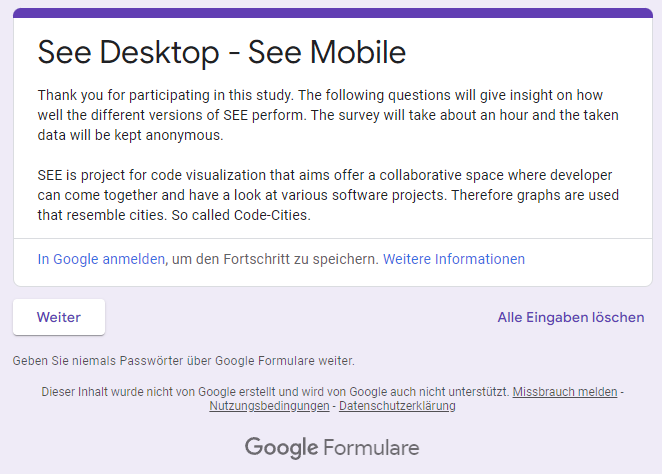
\includegraphics[width=1\textwidth]{Evaluation/img/form_intro.png}
  \caption{The intro of the survey}\label{fig:intro}
\end{figure}

\begin{figure}[H]
  \centering
  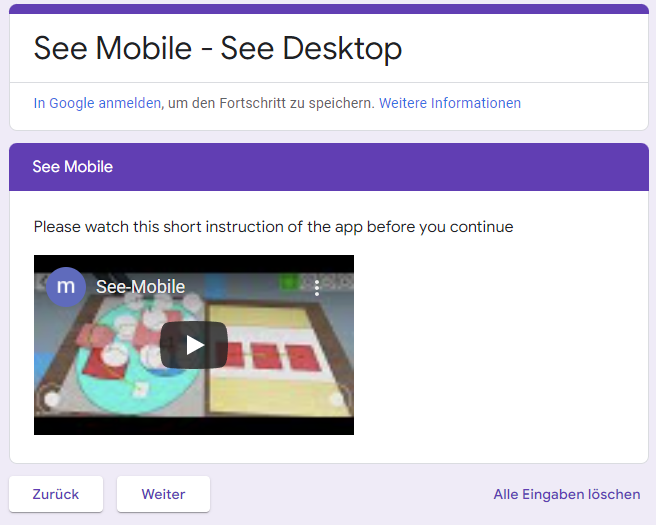
\includegraphics[width=1\textwidth]{Evaluation/img/form_video.png}
  \caption{The introduction video of the survey}\label{fig:video}
\end{figure}

\subsubsection{Questionnaires}
\label{questionaires}
There will be three questionnaires used for the study that will be discussed in detail in the following.
The study will start with a demographic questionnaire that covers general information about the subject.
After every task there will be an \gls{ASQ} and after every block of tasks for each of the two covered devices there will be a \gls{sus} questionnaire.
\paragraph{Demographic questionnaire}\mbox{}\\
The subjects shall start the survey with a demographic questionnaire.
In that section they will be asked for their age, gender, highest degree, experience with \gls{see}, experience with first person video games, their \gls{android} device name, their Android version and their experience with software development.
These specifications will be used to form different groups to see if there is any impact on the result of the following measurements. 
\cite{Mclellan2011} has shown that the user experience can have a significant impact on the \gls{sus}-Score.
It is therefore important to view the measured results in context of the paired demographic data.

The mobile version was only tested on a single \gls{android} device.
It is likely that the performance of the application varies on different \gls{android} versions or devices.

\paragraph{Post-task questionnaire}\mbox{}\\
The \gls{post-task} questionnaire will supplement the \gls{post-study} questionnaire on a micro level.
The main focus here will be on single tasks, which allows to have a look at different aspects like effort, complexity and information provided by the system. 

As a \gls{post-task} questionnaire the \gls{ASQ} will be used. 
The \gls{ASQ} was first introduced in 1991 by \cite{lewis1991psychometric}.
It is designed for task based surveys and contains three questions.
The \gls{ASQ} will be used because it brings the following advantages:
\begin{itemize}
  \item The questionnaire has been used many times over the years and has proven its validity (\cite{hajesmaeel2022most}; \cite{lewis1991psychometric}; \cite{lewis1995ibm}).
  \item With its three questions it is short and does not exhaust the subjects. This is especially important because it will be required to finish this questionnaire a total of four times.
  \item It fits well for this study because it is a questionnaire designed for task based evaluations.
\end{itemize}
The \gls{ASQ} consists of three questions that scale from one to seven, where one means \enquote{strongly disagree} and seven means \enquote{strongly agree}.

\paragraph{Post-study questionnaire}\mbox{}\\
The \gls{post-study} questionnaire is mainly to obtain as much information about the \gls{usability} of the two systems as possible.
The questionnaire can be longer than the \gls{post-task} but still should not be too long to keep the processing time of the survey at around an hour.

The \gls{sus} questionnaire was first published in 1986 by John Brooke (\cite{brooke1996sus}) and is therefore widely used and proven as citations in more than 1200 publications up until 2013 show (\cite{brooke2013}).
The \gls{sus} is used in this study for the following advantages: 
\begin{itemize}
  \item It consists of ten questions and has to be done twice. Twenty questions in total fit well into the planned one hour total time span of this experiment.
  \item It has been made publicly available and is free to use (\cite{brooke1996sus}).
  \item It is widely used and therefore already proven to give useful results (\cite{brooke2013}; \cite{lewis2018system}; \cite{grier2013system}).
  \item According to \cite{doi:10.1177/1541931213571043} and \cite{doi:10.1080/10447310802205776} it is suited to compare two systems.
\end{itemize}
The \gls{sus} questionnaire will contain, as already mentioned, ten questions.
Each question will give a five-level rating from \enquote{strongly disagree} to \enquote{strongly agree}.
The results will then be combined into a \gls{usability}-Score from zero to 100 where a high value represents a good result and a low value a bad one.
\subsubsection{Pilot Study}
\label{pilot}
In a first test, the pilot study was executed with one subject.
Afterward, the study was discussed and checked for errors.
It stood out that the example \gls{city} of task one was too different to the one in the second task.
Therefore, the \gls{city} of the first task was exchanged with a larger and better comparable one.
Further on, a \gls{city} with 1288 nodes (see figure \ref{fig:city2}) as well as one with 1464 nodes (see figure \ref{fig:city3}) will be used.

\begin{figure}[htb]
  \centering
  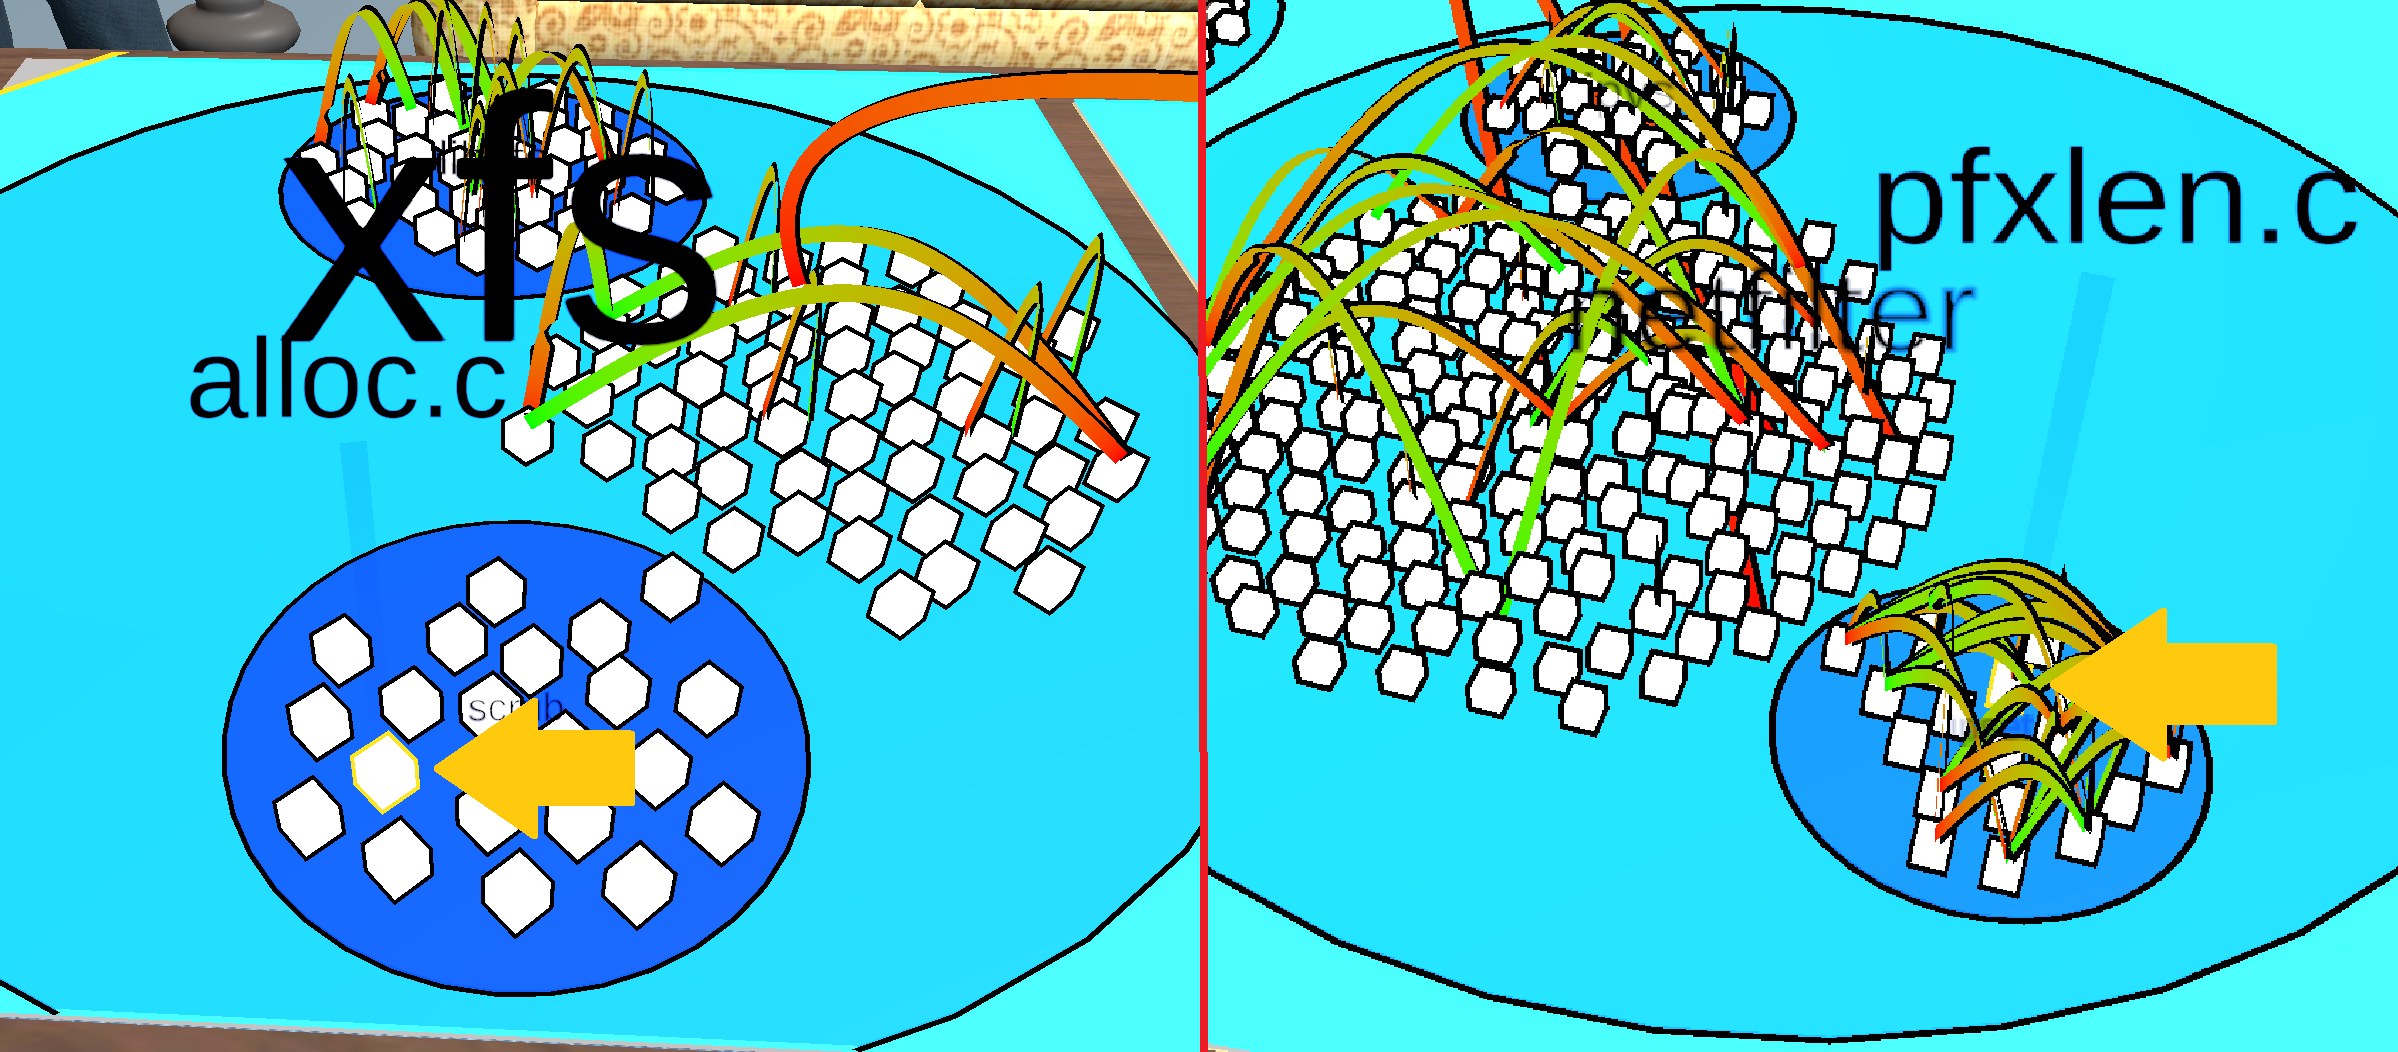
\includegraphics[width=1\textwidth]{Evaluation/img/task1.png}
  \caption{The two key nodes are marked with a yellow arrow}\label{fig:task1}
\end{figure}

Also, the tasks were not comparable because they differed in the types of interactions they used.
In one task the user was asked to rename a node and in the other one the user should have added four nodes.
For renaming a node, the user had to use a keyboard, which does not make it comparable to just click and add nodes in the other task.

To also ensure that task one and task three (first task of each version) are comparable, both tasks are similar in their set-up as seen in figure \ref{fig:task1}.
As one part of the task is to find the right node, both targeted \glspl{node} are on a \gls{plane} with a similar amount of nodes.

The same goes for task three and four (second task of each device) as the target \glspl{plane} that have to be found have a similar size. 
Both tasks also include a hint where to find the desired \glspl{plane}.

\subsubsection{Final Experiment Set Up}
\label{final}
After the pilot study the final set-up can be discussed.
The demographic questionnaires will be designed as described in section \ref{experiment}.
The final questions will be as listed below.
\paragraph{Demographic questions:}
\begin{itemize}
  \item Age
        \begin{itemize}
          \item 0-15 years old
          \item 16-30 years old
          \item 31-45 years old
          \item 46+ years old
        \end{itemize}
  \item What gender do you identify as?
        \begin{itemize}
          \item Male
          \item Female
          \item Other ...
          \item Prefer not to say
        \end{itemize}
  \item What is the highest degree or level of education you have completed?
        \begin{itemize}
          \item Some High School (Hauptschule/Realschule...)
          \item High School (Abitur)
          \item Bachelor's Degree
          \item Master's Degree
          \item Ph.D. or higher
          \item Prefer not to say
          \item Other ...
        \end{itemize}
  \item Questions regarding used hardware and experience
        \begin{itemize}
          \item Are you already experienced with See?
          \item Do or did you play first person video games?
          \item Do or did you develop software?
          \item On which \gls{android} device will you attend?
          \item Which \gls{android} version are you using?*
        \end{itemize}
\end{itemize}

After filling out the demographic questionnaires the subjects will be asked to watch a short tutorial video.
Which video they will watch first will depend on with group they are in.
If they start with the mobile version of \gls{see}, they will be asked to watch \hyperref[calc]{SeeMobile.mp4}, otherwise they will be asked to watch \hyperref[calc]{SeeDesktop.mp4}.
After completing their first training and their first two tasks, as described in table \ref{table:tasks}, they will be asked to watch the video they have not started with.

\begin{table}[htb]
  \resizebox{\textwidth}{!}{%
    \begin{tabular}{lll}
      Nr.                                                                                                                                                                                         &
      Task                                                                                                                                                                                        &
      Expected time                                                                                                                                                                                 \\ \hline
      Training                                                                                                                                                                                    &
      \begin{tabular}[c]{@{}l@{}}Navigate through the Planes "dir\_root" \\ \textgreater "dir\_B" \textgreater "dir\_B\_2". On that Plane \\ select "b2\_b.cpp" and rename it "b42".\end{tabular} &
      1 - 5 mins                                                                                                                                                                                    \\
      1                                                                                                                                                                                           &
      \begin{tabular}[c]{@{}l@{}}Detect the largest Plane "xfs". On that\\ Plane find plane "scrub". Then find \\ and delete node "alloc.c".\end{tabular}                                         &
      0.5 - 5 mins                                                                                                                                                                                  \\
      2                                                                                                                                                                                           &
      \begin{tabular}[c]{@{}l@{}}Find the Plane with one blue child \\ Plane ("btrfs"). On the blue child \\ Plane "tests" add four new nodes.\end{tabular}                                       &
      1 - 5 mins                                                                                                                                                                                    \\ \hline
      Training                                                                                                                                                                                    &
      \begin{tabular}[c]{@{}l@{}}Navigate through the Planes "dir\_root" \\ \textgreater "dir\_C" \textgreater "dir\_C\_2". On that Plane \\ select "c2\_b.cpp" and rename it "c42".\end{tabular} &
      1 - 5 mins                                                                                                                                                                                    \\
      3                                                                                                                                                                                           &
      \begin{tabular}[c]{@{}l@{}}Detect the \\ largest Plane "netfilter". On that Plane\\ find Plane "ipset". Then find and \\ delete node "pfxlen.c".\end{tabular}                               &
      0.5 - 5 mins                                                                                                                                                                                  \\
      4                                                                                                                                                                                           &
      \begin{tabular}[c]{@{}l@{}}On the Plane with the most \\ edges ("ipv6") find the smallest Plane\\ "ila" and connect all four nodes on it.\end{tabular}                                      &
      1 - 5 mins                                                                                                                                                                                    \\ \hline
    \end{tabular}%
  }
  \caption{The tasks used for the experiment. The device will be switched after task 2.}
  \label{table:tasks}
\end{table}

After each task, the subjects will be asked to fill out an \gls{ASQ} and after each block of task, as described in table \ref{table:procedure}, they will be asked to fill out a \gls{sus} questionnaire.
Therefore, each participant has to fill out four \glspl{ASQ} and two \gls{sus} questionnaires.
The full study should not take longer than an hour.

\begin{table}[htb]
  \resizebox{\textwidth}{!}{%
    \begin{tabular}{llll}
      Phase          &                        & \multicolumn{2}{l}{Description}                                          \\ \hline
      Pre-Experiment &                        & \multicolumn{2}{l}{Demographic questionnaire}                            \\ \hline
                     & City                   & Group 1                                       & Group 2                  \\ \hline
      Training       & Figure \ref{fig:city1} & \multirow{6}{*}{Desktop}                      & \multirow{6}{*}{Mobile}  \\
      Task 1         & Figure \ref{fig:city2} &                                               &                          \\
      ASQ            &                        &                                               &                          \\
      Task 2         & Figure \ref{fig:city2} &                                               &                          \\
      ASQ            &                        &                                               &                          \\
      SUS            &                        &                                               &                          \\ \hline
      Training       & Figure \ref{fig:city1} & \multirow{6}{*}{Mobile}                       & \multirow{6}{*}{Desktop} \\
      Task 3         & Figure \ref{fig:city3} &                                               &                          \\
      ASQ            &                        &                                               &                          \\
      Task 4         & Figure \ref{fig:city3} &                                               &                          \\
      ASQ            &                        &                                               &                          \\
      SUS            &                        &                                               &
    \end{tabular}%
  }
  \caption{Experimental procedure per subject. The procedure is swapped per group.}
  \label{table:procedure}
\end{table}


\subsubsection{Execution}
Before the study, the subjects got an installation instruction as well as the two applications.
For the execution of the user study, every subject got one of two links to a Google form.
Each form starts with a different device. 
The forms were handed out in alternating order and the subjects should therefore be randomly assigned to the two groups.

The study was executed within a week and a total of 20 subjects participated.
From the 20 subjects, two could not finish the tasks on their mobile device, which leaves n = 18 participants that finished the survey.

The instance of \gls{see} was hosted from the home network of the overseer. 
The overseer also watched the subjects doing their task.
The subjects got instructions for the training tasks, and it was ensured that all essential interactions were trained such as zooming and moving the \gls{city}.
Every subject got the same base training, but was allowed to ask further questions or try out other interactions.


\subsection{Results}
The \hyperref[calc]{calc\_data.ipynb} script can be used to reproduce the result data for the following section.
Also, all shown diagrams in this section can be reproduced with the script.

In the following, the group that started the study with the desktop version of \gls{see} will be called \textit{Group 1} and the group that started with the mobile version will be called \textit{Group 2}.
The task order of the two groups remains the same.
Both groups start with the same task.
That way not only both groups but also the desktop and the mobile \gls{see} version will be compared. 

In the coming up section the \gls{utest} will be used multiple times to see if there are significant differences between two data sets.
The \gls{utest} brings the advantage that the tested data sets do not need to fulfill the requirement of a normal distribution (\cite{gibbons1991comparisons}).
This is important because the sample size of n = 18 is too small to assume a normal distribution.
The used level of significance will be $\alpha = 0.05$.

\label{results}
\subsubsection{Demographic Data}
\label{sec:demo}
In this subsection it will be verified if the two groups differ significantly in their demographic data. 
Therefore, a two-tailed \gls{utest} that checks whether a set of demographic values from \textit{Group 1} $\neq$  a set of demographic values from \textit{Group 2}, will be used.
Both groups have a sample size of $n = m = 9 $ with $\alpha = 0.05$ which leads to a critical value of $U = 17$ for a two-tailed \gls{utest} (\cite{zar2010biostatistical}).

\paragraph{Gender}\mbox{}\\
Of 18 participants, 17 reported being male. 
One participant preferred not to say their gender and can therefore not be grouped.
Due to this fact, a grouping does not make sense here in general. 

\paragraph{Age}\mbox{}\\
The subjects were asked to choose their age in grouped options. 
Most of the participants were aged between 16 and 30 years.
Only two participants were aged between 31 and 45 years. 
Therefore, the age of the participants should not fall into account of the results of the study.

\paragraph{Highest degree}\mbox{}\\
Nine of the participants answered with \enquote{Bachelor's Degree} for their highest achieved degree. 
It is therefore the most common option as illustrated in figure \ref{fig:degree}.

To measure the \gls{utest}, the options were put into an ordinal scale which follows the same order as in the survey.
The test shows that there is no significant difference between the two groups ($U = 33.0; p \approx 0.51$).

\begin{figure}[H]
  \centering
  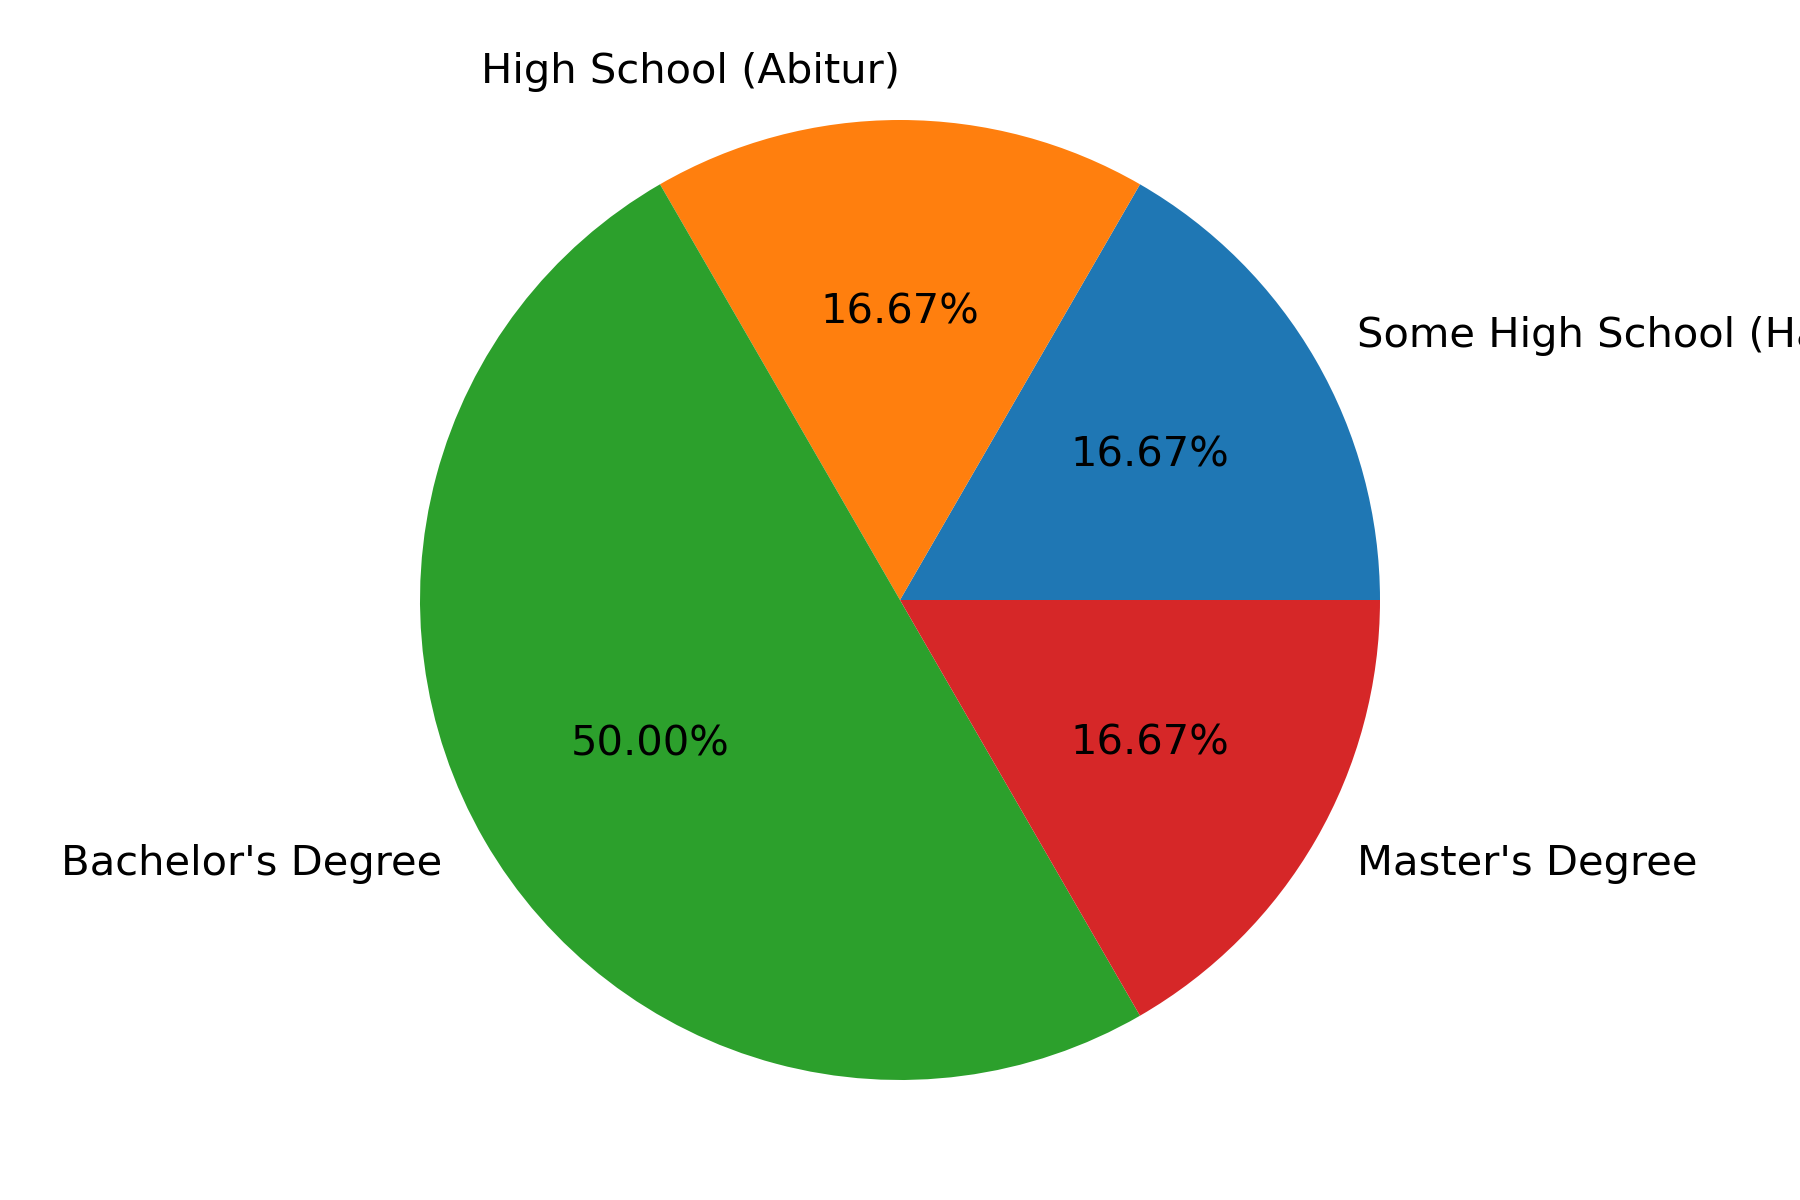
\includegraphics[width=0.7\textwidth]{Evaluation/img/degree.png}
  \caption{The distribution of the highest completed degrees of all 18 subjects}\label{fig:degree}
\end{figure}

\paragraph{Experience}\mbox{}\\
The subjects were asked if they had experience regarding \gls{see}, software development and first person video games.
All but one subject had experience with first person video games and the single subject without experience had at least experience with \gls{see} which could arguably count as a first person video game.
Therefore, experience with first person video games should not have impact on this study.

Five of 18 subjects had experience with \gls{see}.
The \gls{utest} shows there is no significant difference between the two groups ($U = 27.0; p \approx 0.23$).
Even though there is no significant difference, four of the subjects with \gls{see} experience are in \textit{Group 2} and only one in \textit{Group 1}.

The majority of ten subjects had experience with software development.
The other eight subjects had no experience.
The \gls{utest} shows there is no significant difference between the two groups ($U = 49.5; p \approx 0.38$).

\paragraph{Android device and version}\mbox{}\\
A large variety of 17 different \gls{android} devices were used.
Therefore, the distribution of \gls{android} devices should not have impact on the study results.
Nonetheless, it has to be considered that the devices \enquote{Huawei P10 lite}, \enquote{Huawei P20 Pro} \enquote{Samsung A52S}, \enquote{Samsung S9} and the \enquote{Poco X3 Pro} had performance issues.
These performance issues showed in bumpy movement and player interactions.
Unfortunately, it could not be measured how strong the impact was on the performance on the single phones.
The threats of validity this could cause will be further discussed in section \ref{sec:validity}.
Three of the devices with bad performance belong to \textit{Group 1} and the other two to \textit{Group 2}.

There was not as much variety in the used \gls{android} version as it was with used \gls{android} devices. 
The most commonly used one was \gls{android} 12, which is also the most current one to the time of this writing.
\gls{android} 12 was used by seven subjects.
The second most used version was \gls{android} 11.
One subject used \gls{android} 7 on the \enquote{Huawei P10 lite}.
This is remarkable because \gls{android} 7 was released in 2016\footnote{\url{https://android-developers.googleblog.com/2016/08/taking-final-wrapper-off-of-nougat.html} (10.06.2022, 12:37)} and the \enquote{Huawei P10 lite} was released a little later in March 2017\footnote{\url{https://www.gsmarena.com/huawei_p10_lite-8598.php} (10.06.2022, 12:37)} but \gls{see} still managed to work, even if with lower performance.
The distribution of the used \gls{android} devices can be seen in figure \ref{fig:android_version}.
The \gls{utest} shows there is no significant difference between the two groups ($U = 39.0; p \approx 0.93$).

\begin{figure}[htb]
  \centering
  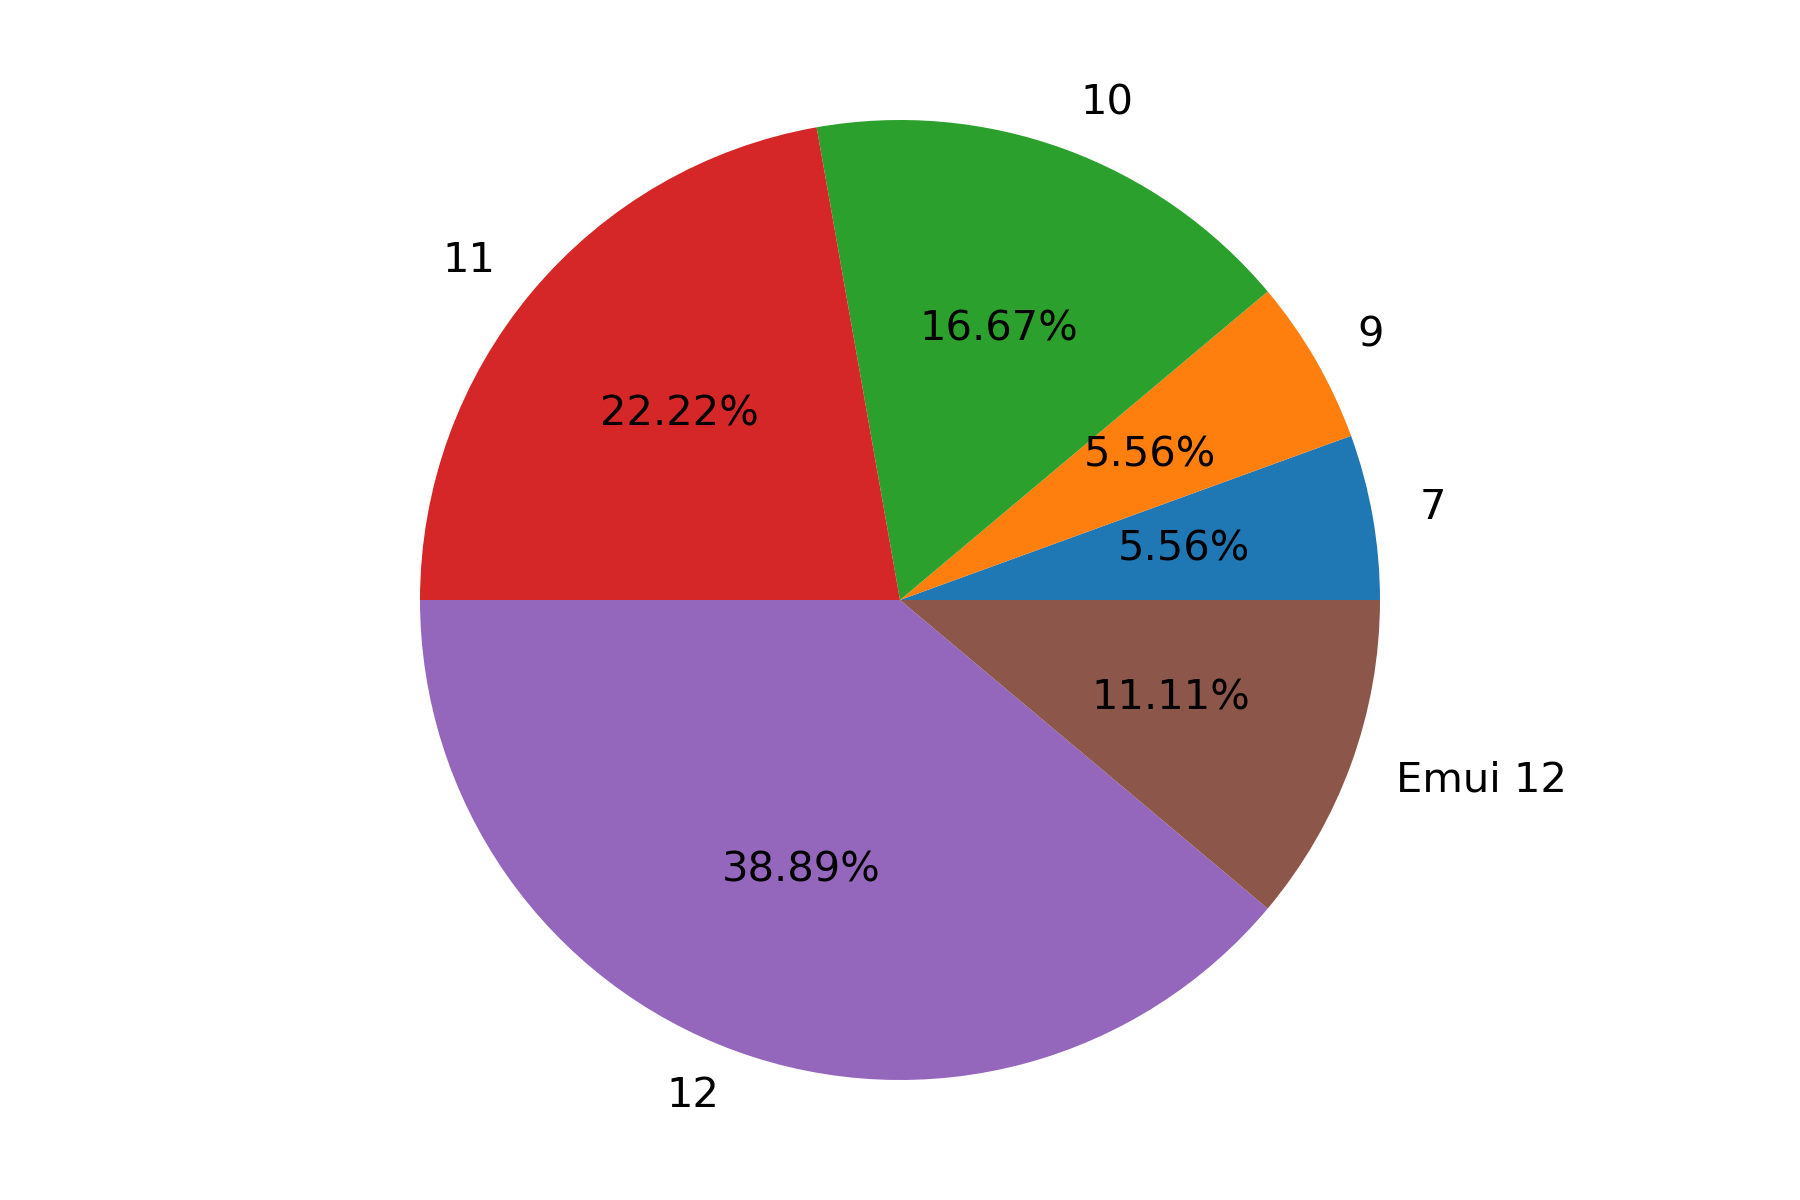
\includegraphics[width=0.7\textwidth]{Evaluation/img/droid_version.png}
  \caption{The distribution of the Android versions the subjects were using}\label{fig:android_version}
\end{figure}

\mbox{}\\
Surprisingly, there has been no significant difference with the demographic data between the two groups.
In the following section the more exciting data will be analyzed. 

\subsubsection{Performance}
For the \textit{performance} aspect, the time needed for each task was measured.
The time for the trainings task however was not measured because it would not fit the purpose of a training to be measured by time.
Therefore, the overseer asked the subjects to tell when they begin the task. 
The time was taken after the subject has read and understood the task, and it was stopped when the subject successfully finished.
This will help to prove or discard hypothesis $H_{a}$.

In the following, the two groups in general will be in focus.
Is there any significant difference?
The total time needed for all subjects in the two groups can be seen in figure \ref{fig:group_time_violin}.
The average time \textit{Group 1} needed to complete all tasks was $\overline{t_1} = 487s$ and for \textit{Group 2} it was $\overline{t_2} = \approx388s$.
The median time for \textit{Group 1} was $\widetilde{t1} = 315s$ and for \textit{Group 2} it was $\widetilde{t_2} = 384s$.
As figure \ref{fig:group_time_violin} shows and the values mentioned above suggest the \gls{utest} shows there is no significant difference between the two groups with a $U = 43.0$ and $p \approx 0.86$.

\begin{figure}[htb]
  \centering
  \includegraphics*[width=1\textwidth]{Evaluation/img/group_time_violin.png}
  \caption{Total time each group needed as violin plot}
  \label{fig:group_time_violin}
\end{figure}

Furthermore, a look at the single tasks will be taken. 
Has there maybe been a learning effect or difference in general between the groups? 
To find out task 1 from \textit{Group 1} will be compared with task 3 from \textit{Group 2} and so on.
Every pair of tasks is comparable because they have been done on the same device and use the same set of user interactions as described in section \ref{final}.
The \gls{utest} shows that there is no significant difference in any combination as listed below:
\begin{itemize}
  \item \textit{Group 1}, task 1 \& \textit{Group 2}, task 3: $U = 26.5; p \approx 0.23$
  \item \textit{Group 1}, task 2 \& \textit{Group 2}, task 4: $U = 35.5; p \approx 0.69$
  \item \textit{Group 1}, task 3 \& \textit{Group 2}, task 1: $U = 49.0; p \approx 0.48$
  \item \textit{Group 1}, task 4 \& \textit{Group 2}, task 2: $U = 57.0; p \approx 0.16$
\end{itemize}

Finally, the question, if there is a significant difference between the two used versions of \gls{see} in the single tasks, will be looked at.
The time needed for every single task on both versions can be seen in figure \ref{fig:speed_violin}.
There are some results that stand out and took way longer than the medians would suggest.
That could be caused by various reasons as for example:
\begin{itemize}
  \item The mobile version of \gls{see} did not run smoothly on the subjects device and therefore the tasks became harder.
  \item The subject did not understand the task correctly and had to reread it.
  \item The subject overlooked a key object and continued the search at wrong areas.
\end{itemize}

\begin{sidewaysfigure}
  \centering
  \includegraphics*[width=1.15\textwidth]{Evaluation/img/speed1_violin.png}
  \caption{Violin plots of all tasks by device}
  \label{fig:speed_violin}
\end{sidewaysfigure}

To prove the hypothesis $H_a$, every task will be checked if the subjects needed significantly less time with the desktop version of \gls{see} than with the mobile version.
Therefore, a one-sided \gls{utest} will be used.
The critical value here is $U = 21$.

\begin{description}
  \item[Task i] The subjects needed an average time of $\approx 80s$ with the desktop version and $\approx 166s$ with the mobile version. 
  The median here was 47s with the desktop version and 150s with the mobile version. 
  The medians show that there are some outliers on both sides that took longer than the usual subject needed. 
  The one-sided \gls{utest} shows, with $U = 19; p \approx 0.03$, that the subjects needed significantly less time with the desktop version than with the mobile version.
  \item[Task ii] This task shows the lowest notable difference in figure \ref{fig:speed_violin}. 
  The \gls{utest} shall confirm this assumption with $U=24; p \approx 0.08$.
  This results shows that the subjects did not need significantly less time to solve task 2 with the desktop version than with the mobile version.
  The average time of the desktop version here is $\approx 47s$ and of the mobile version $\approx 74$, while the desktop median lays at $57s$ and the mobile median at $67s$.
  \item[task iii] In contrast to task 2, this task shows the biggest difference in figure \ref{fig:speed_violin} and once again the one-sided \gls{utest} approves this clearly with a result of $U=12.0;p \approx 0.007$. 
  This shows that the desktop version needed significantly less time than the mobile version once more. 
  Also, the average time needed spreads quite far with an average of $\approx 82s$ for the desktop version and $\approx 247s$ for the mobile version.
  The median values are 77s for the desktop version and 151s for the mobile version.
  The desktop median is almost the same as the desktop average while the mobile median is again quite far from the average, which shows that there are again some outliers that took much longer than the usual subject. 
  This could, among other things, be caused by the reported bad performance of the devices \enquote{Huawei P20 Pro} and \enquote{Huawei P10 Lite}, which were used for task 3.
  \item[Task iv] The average time needed to complete the task was $\approx 67s$ for the desktop version and $\approx 113s$ for the mobile version. 
  The medians here were 46s for the desktop version and 111s for the mobile version. 
  The values differ quite much and the \gls{utest} validates one last time that the desktop version needed significantly less time than the mobile version to complete the tasks ($U=17.5;p \approx 0.023$).
\end{description}

To close this section, figure \ref{fig:device_time_violin} shows the total time needed for all tasks by used device.
The one-sided \gls{utest} for the alternative hypothesis has a clear result of $U=11.0$ and $p \approx 0.996$.
Therefore, the alternative hypothesis $H_a0:$ \enquote{The time required in {\gls{see}} desktop is lower than the time required in \gls{see} mobile} cannot be rejected, and the null hypothesis can be assumed false.

\begin{figure}[htb]
  \centering
  \includegraphics*[width=1\textwidth]{Evaluation/img/device_time_violin.png}
  \caption{Total time the subjects needed on the different devices as violin plot}
  \label{fig:device_time_violin}
\end{figure}

Summarized it can be said that the subjects were faster on the desktop version of \gls{see}.
All data sets regarding the required time to solve the four tasks are comparable, even crossed over like for example task 1 and task 3. 
Only for one task the subjects did not need significantly less time on the desktop version, but the border value to a significant result was quite close.
All in all, the desktop version did perform better than the mobile version regarding the required time.

\subsubsection{Usability}
\label{sec:usability}
This section will discuss the results of the \gls{usability} questionnaires presented in section \ref{questionaires}.
First the \gls{ASQ} results will be analyzed and second the \gls{sus} results to test the hypotheses that were presented in section \ref{aim}.

\paragraph{ASQ}\mbox{}\\
As a start, the \gls{post-task} questionnaire will be looked at. 
Figure \ref{fig:asq_group} shows the ASQ results by group, independent of the used device.
Unfortunately, the results differ significantly as the \gls{utest} shows with $U=392.5$ and $p \approx 0.0037$.
Therefore, a deeper look is needed. 
The results of \textit{Group 1} do not differ significantly from \textit{Group 2}, looking only at the tasks completed with the desktop device, as the \gls{utest} shows with $U=122.5$ and $p \approx 0.21$.
In opposition, the results only caused by completing tasks with a mobile device differ significantly as the \gls{utest} shows ($U=73.0;p \approx 0.0048$).
Having another look at figure \ref{fig:asq_group}, the result of \textit{Group 1} with the mobile device stands out. 
Comparing the two groups without the described results of \textit{Group 1} results in a \gls{utest} of $U=266.5; p \approx 0.29$, which means without the subset of \textit{Group 1} the two groups show no significant difference.

\begin{sidewaysfigure}
  \hspace*{-1.5in}
  \centering
  \includegraphics*[width=1.15\textwidth]{Evaluation/img/group_asq_violin.png}
  \caption{Violin plots of all tasks by group}
  \label{fig:asq_group}
\end{sidewaysfigure}

To ensure a good comparability further on all tasks will be looked at separately. 
The \gls{ASQ} consists of three questions, each representing a different aspect.
In the following, all tasks will be compared as shown in table \ref{table:asq_combi}.

\begin{table}[htb]
  \resizebox{\textwidth}{!}{%
  \begin{tabular}{lllll}
    ASQ Question                        & \multicolumn{4}{l}{Complexity}  \\ \hline
    \multicolumn{1}{l|}{Group 1, Task:} & 1       & 2     & 3     & 4     \\
    \multicolumn{1}{l|}{Group 2, Task:} & 3       & 4     & 1     & 2     \\
    \multicolumn{1}{l|}{Mann-Whitney-U} & $U=47 ;p \approx 0.58$ & $U=37.5;p \approx 0.81$ & \cellcolor[HTML]{FFFC9E} $U=7.0;p \approx 0.003$  & $U= 24.5;p \approx 0.16$      \\ \hline
    ASQ Question                        & \multicolumn{4}{l}{Effort}      \\ \hline
    \multicolumn{1}{l|}{Group 1, Task:} & 1       & 2     & 3     & 4     \\
    \multicolumn{1}{l|}{Group 2, Task:} & 3       & 4     & 1     & 2     \\
    \multicolumn{1}{l|}{Mann-Whitney-U} & $U= 44;p \approx 0.78$        & $U=37 ;p \approx 0.78$      & \cellcolor[HTML]{FFFC9E} $U= 13.5;p \approx 0.02$      & $U= 23;p \approx 0.11$      \\ \hline
    ASQ Question                        & \multicolumn{4}{l}{Information} \\ \hline
    \multicolumn{1}{l|}{Group 1, Task:} & 1       & 2     & 3     & 4     \\
    \multicolumn{1}{l|}{Group 2, Task:} & 3       & 4     & 1     & 2     \\
    \multicolumn{1}{l|}{Mann-Whitney-U} & $U= 39.5;p \approx 0.96$ & $U= 36;p \approx 0.70$      & $U= 20.5;p \approx 0.07$      & $U= 20.5;p \approx 0.07$     
    \end{tabular}%
  }
  \caption{Two-sided \gls{utest} for each comparable question on the same device.}
  \label{table:asq_combi}
  \end{table}

The two marked \glspl{utest} in table \ref{table:asq_combi} show that the pair \textit{Group 1, Task 3 - Group 2, Task 1 - ASQ Question 1} as well as \textit{Group 1, Task 3 - Group 2, Task 1 - ASQ Question 2} have significant differences.
As those two pairs are not comparable, they will not be observed further on.
All remaining results can be seen in figure \ref{fig:effort_violin} for the \gls{ASQ} aspect \textit{effort}, in figure \ref{fig:complexity_violin} for \gls{ASQ} aspect \textit{complexity} as well as in figure \ref{fig:info_violin}, which covers the \gls{ASQ} aspect \textit{information}.

\begin{figure}[htb]
  \hspace*{-1.4in}
  \centering
  \includegraphics*[width=1.4\textwidth]{Evaluation/img/effort_violin.png}
  \caption{ASQ effort results violin plots of all tasks by device}
  \label{fig:effort_violin}
\end{figure}

\begin{figure}[htb]
  \hspace*{-1.4in}
  \centering
  \includegraphics*[width=1.4\textwidth]{Evaluation/img/complexity_violin.png}
  \caption{ASQ complexity results violin plots of all tasks by device}
  \label{fig:complexity_violin}
\end{figure}

\begin{sidewaysfigure}
  \hspace*{-1.5in}
  \centering
  \includegraphics*[width=1.15\textwidth]{Evaluation/img/information_violin.png}
  \caption{ASQ information results violin plots of all tasks by device}
  \label{fig:info_violin}
\end{sidewaysfigure}

The \gls{utest} only shows significant findings for two tasks:
\begin{description}
  \item[Task iii] The desktop version of \gls{see} has significant better results than the mobile version in the aspect of information. 
  The subjects rated the desktop version with an average score of 6.22 and a median score of 7, while the mobile version was rated an average of 6.44 and a median of 5.22.
  The \gls{utest} results here are $U = 20.5$ and $p \approx 0.037$.
  \item[Task iv]  The desktop version also showed better results for the aspect of information in this task. 
  The subjects rated the desktop version with an average score of 6.44 and a median of 7, while the mobile version was rated with an average of 5.22 and a median of 6. 
  The \gls{utest} resulted in $U=20.5$ and $p \approx 0.035$ in a one-sided test, which means the desktop version got a significantly higher rating than the mobile version.
\end{description}

All other tasks show no significant higher or lower results. 
It is also to mention that the desktop version only scored a significant higher value at the aspect of information.
That was to be expected because the mobile versions offer less information due to its constrains regarding the screen size. 
The mobile version uses for example only icon buttons and not text buttons like the desktop version, which saves screen space but sacrifices information value, since the user has to remember the meaning of each icon.

Finally, the hypotheses $H_b$, $H_c$, $H_d$ can be rated:

\begin{description}
  \item[$H_b$] The null hypothesis $H_{b0}$ can not be rejected, since the \gls{utest} results in $U = 362.0; p \approx 0.23$. 
  This means that the desktop score for the \gls{ASQ} aspect \textit{complexity} is not significantly higher than the score for the mobile version. 
  \item[$H_c$] The same goes for null hypothesis $H_{c0}$. 
  It can not be rejected, since the \gls{utest} results in $U = 348.5; p \approx 0.32$.
  That means that the desktop \gls{ASQ} score for the aspect \textit{effort} is also not significantly higher than the mobile \gls{ASQ} score.
  \item[$H_d$]  Two of the four tasks showed a significantly higher score for the desktop version in the \gls{ASQ} aspect \textit{information}, but for all four tasks combined the null hypothesis $H_{d0}$ can not be rejected, since the \gls{utest} resulted $U = 776.5; p \approx 0.06$.
  The results are notably close to the significance level of $\alpha = 0.05$ in this example.
 \end{description}

 The final ASQ scores, which are an average of all three questions, can be found in table \ref{table:asq}.
 However, the final ASQ-Scores still differ significantly as the \gls{utest} of $U=92.0; p \approx 0.03$ shows.
 Since, even after not taking into account the previously discussed pairs of tasks, the \gls{ASQ} scores of the two groups differ significantly, which means the final scores cannot be compared.

\begin{table}[htb]
  \resizebox{\textwidth}{!}{%
  \begin{tabular}{l|l|l|l|l|l|l|l|l|l|l|l|l|l|l|l|l|l|l}
  D & 5.8 & 4.7 & 6.3 & 5.2 & 6.8 & 5.8 & 6.7 & 6.3 & 4.8 & 6.7 & 6.7 & 5.8 & 5.3 & 6.8 & 5.0 & 6.5 & 6.8 & 6.3 \\
  M & 6.8 & 6.8 & 6.0 & 6.8 & 6.3 & 4.0 & 6.0 & 7.0 & 6.3 & 6.3 & 5.0 & 6.0 & 5.3 & 5.3 & 2.3 & 7.0 & 5.3 & 3.0
  \end{tabular}%
  }
  \caption{The \gls{ASQ}-scores from all 18 subjects. The first row contains the \gls{ASQ}-scores for the desktop application and the second row for the mobile application. The figures have been rounded to whole numbers.}
  \label{table:asq}
\end{table}

In summary, it can be said that the \gls{ASQ} results show that the two versions of \gls{see} show little significant difference. 
In total only task 3 and task 4 showed a significant difference in favor of the desktop version for the \gls{ASQ} aspect \textit{information}.
\paragraph{SUS}\mbox{}\\
Last but not least, the results of the \gls{sus} questionnaire will be discussed.
The \gls{sus} questionnaire results in a \gls{sus}-Score which was calculated by the formula of \cite{lewis2018system}:

\begin{equation}
SUS = 2.5 \cdot (20 + \sum_{i=1}^1 (-1)^{i+1} \cdot S_i)
\end{equation}

In this formula $S_i$ is the score of one of the ten questions in the \gls{sus}. 
The question scores are alternating positive and negative for the \gls{sus} score.
Therefore, the factor $(-1)^{i+1}$ is needed to either add or subtract from the final \gls{sus} score.

The \gls{sus} scores from both groups can be seen in table \ref{table:sus}.
Both groups can be compared, as the \gls{utest} shows with a result of $U=106.0; p \approx 0.08$. 
The group results can also be seen visualized as violin plots in figure \ref{fig:sus-group-vio}.
The average score of \textit{Group 1} was $ \approx 60.83$ and the score of \textit{Group 2} was $\approx 72.77$.
The median of \textit{Group 1} was 58.75 and of \textit{Group 2} it was 82.5.
The median of \textit{Group 2} differs quite much from the average which indicates an uneven distribution and outliers that are lower than normal.
This can also be seen in figure \ref{fig:sus-group-vio}.

\begin{table}[htb]
  \resizebox{\textwidth}{!}{%
  \begin{tabular}{l|l|l|l|l|l|l|l|l|l|l|l|l|l|l|l|l|l|l}
  D & 60 & 58 & 80 & 60 & 78 & 70 & 85 & 53 & 80 & 88 & 80 & 50 & 63 & 85 & 50 & 93 & 100  & 85 \\
  M & 38 & 53 & 83 & 53 & 53 & 30 & 88 & 35 & 43 & 86 & 48 & 48 & 55 & 90 & 50 & 88 & 98 & 58
  \end{tabular}%
  }
  \caption{The \gls{sus}-scores from all 18 subjects. The first row contains the \gls{sus}-scores for the desktop application and the second row for the mobile application. The figures have been rounded to whole numbers.}
  \label{table:sus}
\end{table}

\begin{figure}[htb]
  \centering
  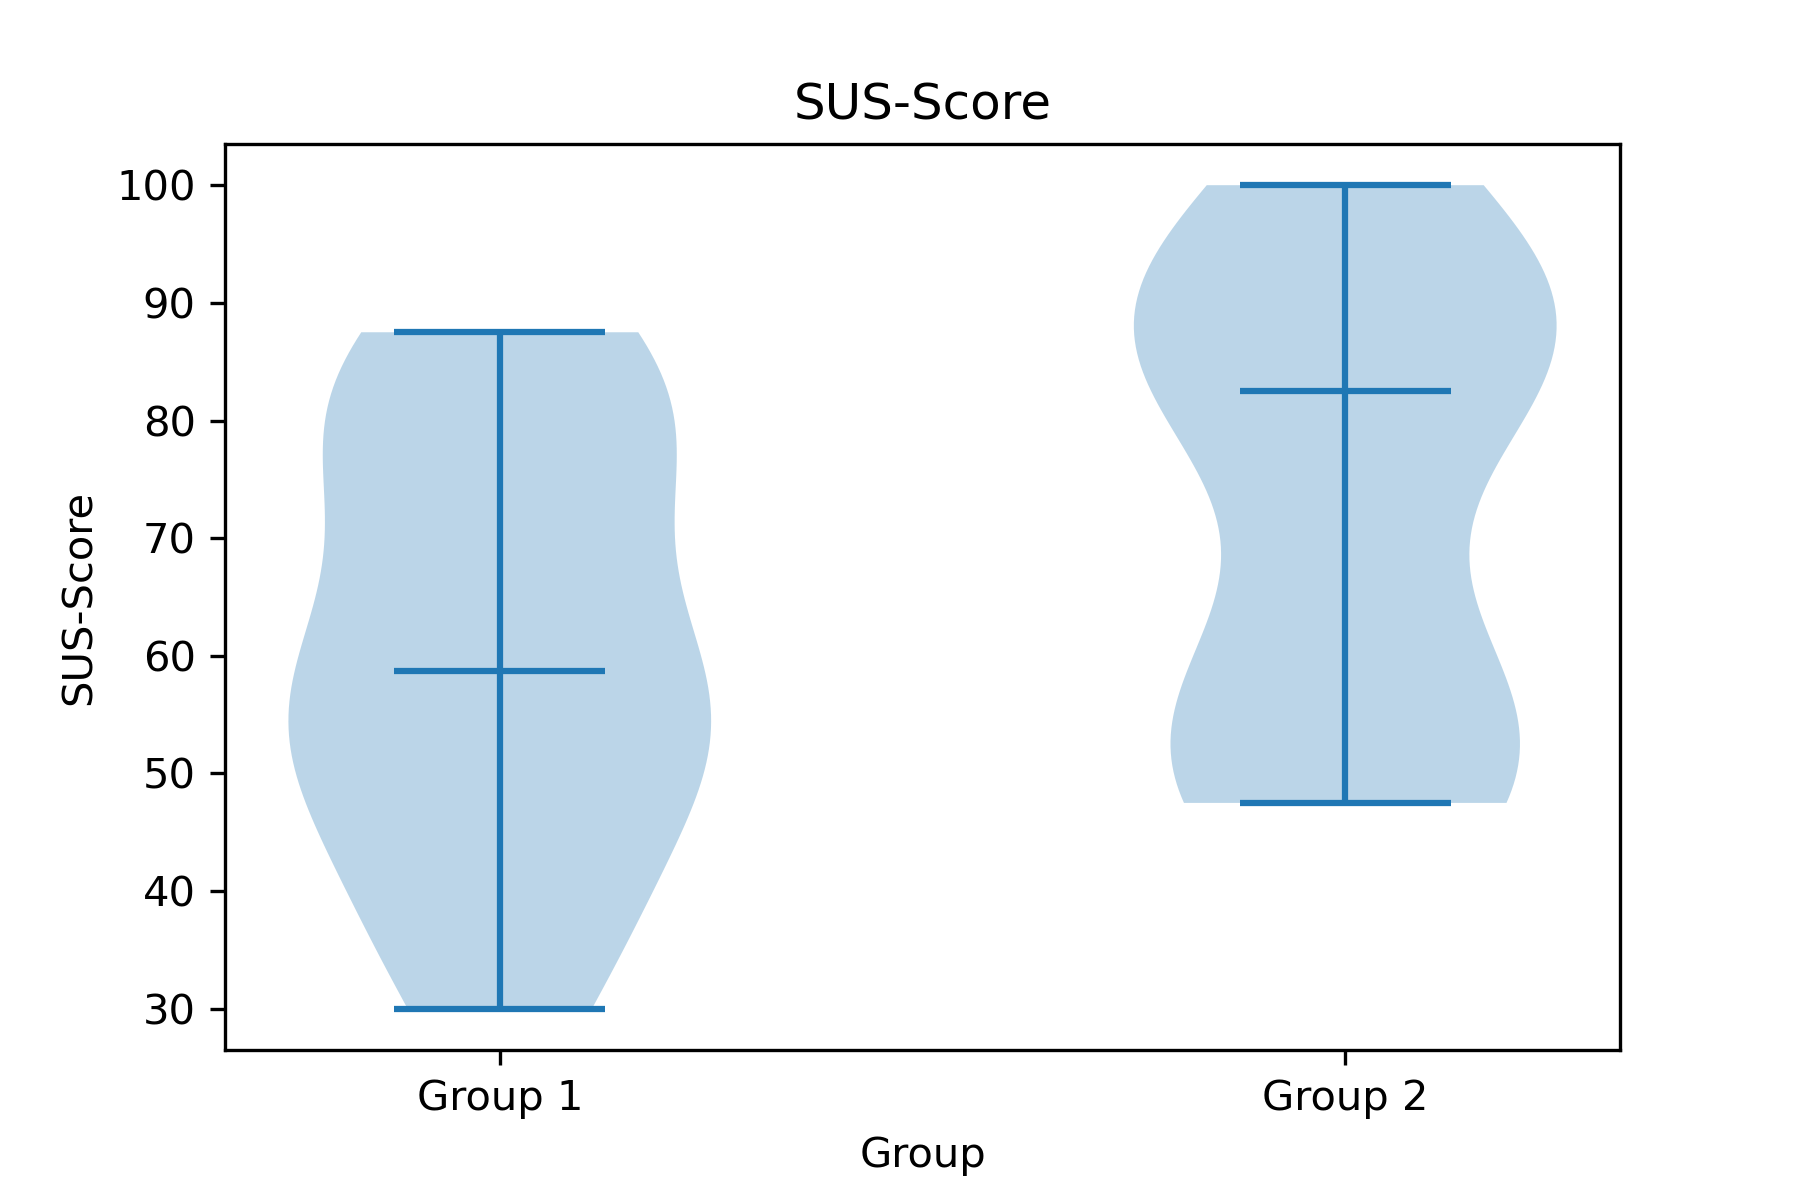
\includegraphics[width=1\textwidth]{Evaluation/img/SUS-Score_group_violin.png}
  \caption{The SUS-Scores of the two \gls{see} versions by group}\label{fig:sus-group-vio}
\end{figure}

Finally, comparing the \gls{sus}-Scores (figure \ref{fig:sus-vio}) of the two different versions shows that the null hypothesis $H_{e0}$ can be rejected, since the \gls{utest} resulted in $U = 219.5; p \approx 0.035$.
The desktop version had an average \gls{sus}-Score of $\approx 73.06$ and a median of 78.75, while the mobile version had an average \gls{sus}-Score of $\approx 60.56$ and a median of 52.5. 
After seeing the results, it can be assumed that the \gls{usability} of the desktop version is significantly higher than the \gls{usability} of the mobile version.
\begin{figure}[htb]
  \centering
  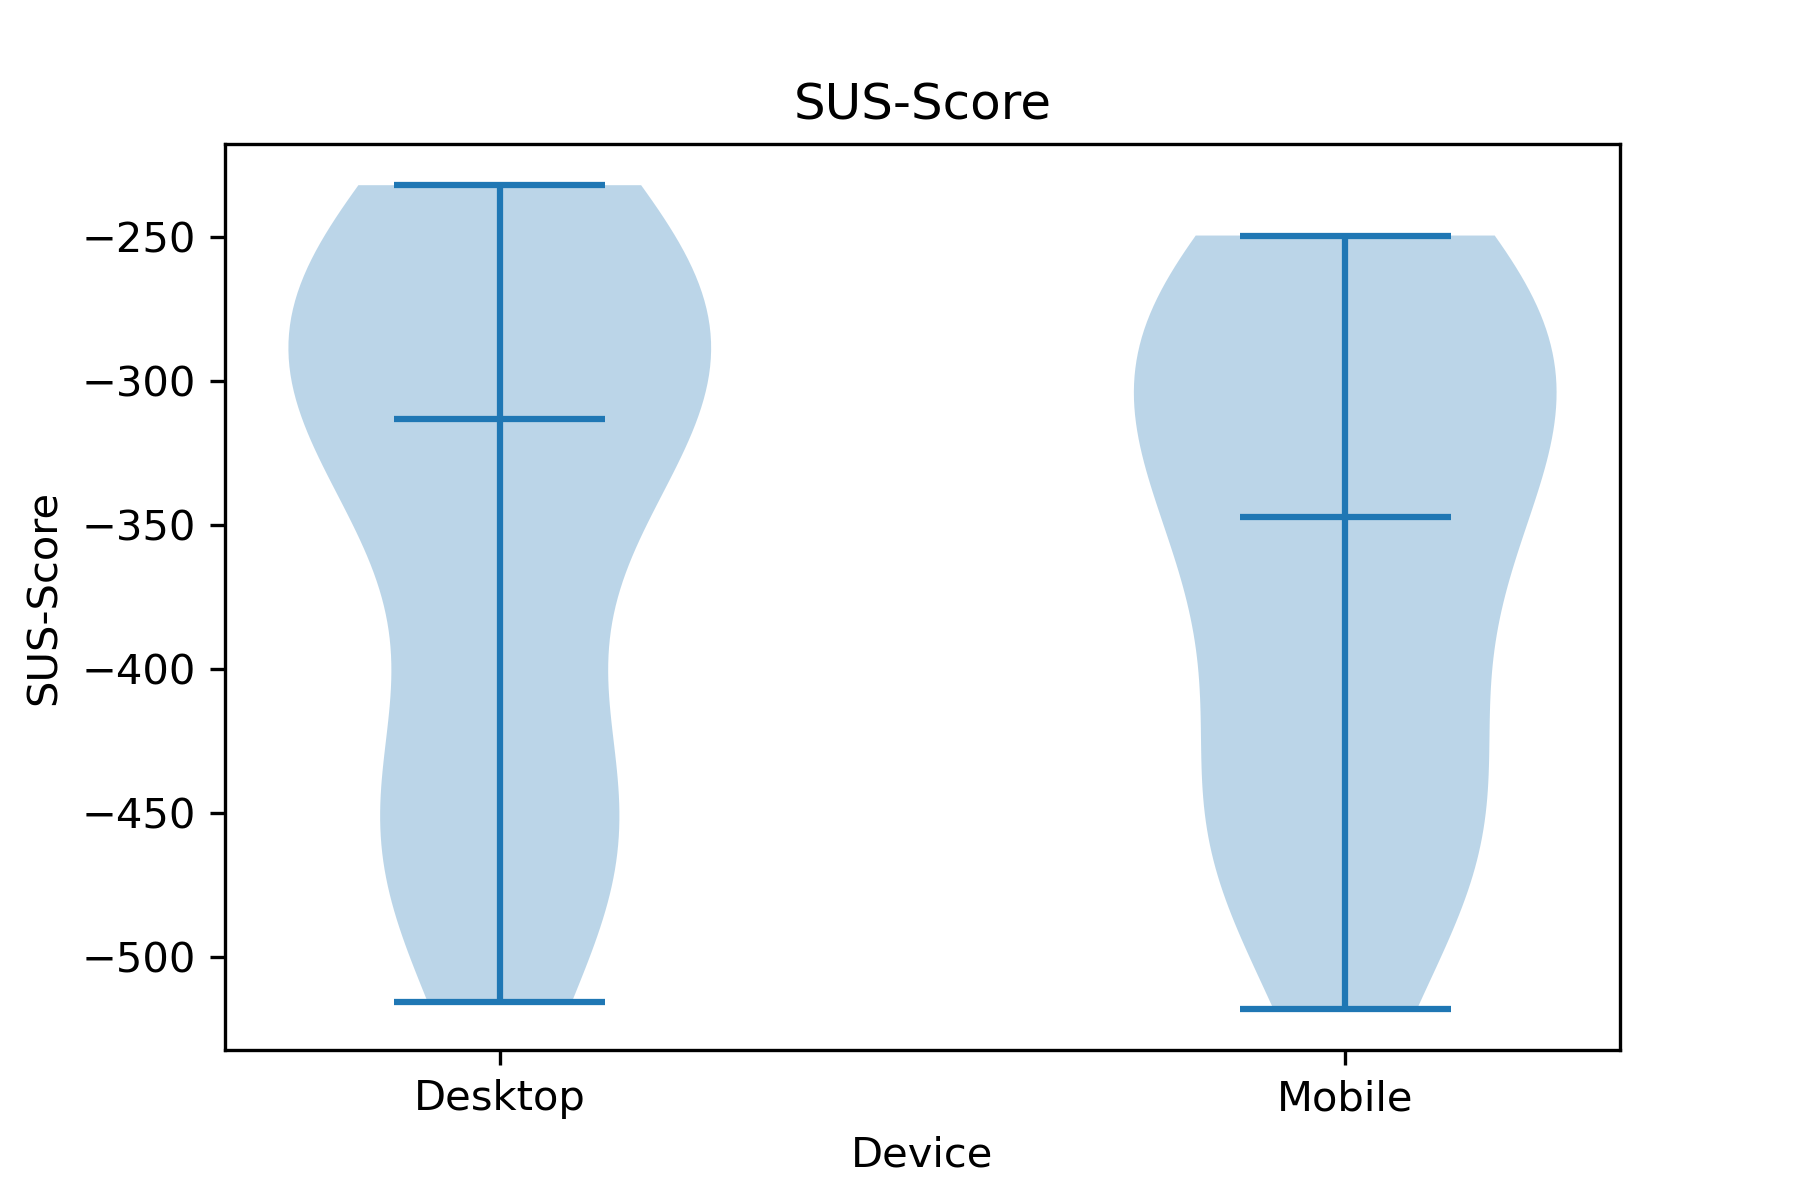
\includegraphics[width=1\textwidth]{Evaluation/img/SUS-Score_violin.png}
  \caption{The SUS-Scores of the two \gls{see} versions by device}\label{fig:sus-vio}
\end{figure}

\subsubsection{Impact of Experience}
\label{sec:experinece}
As already described in section \ref{aim}, the subjects will be grouped by their level of experience and their results will be analyzed.
Since only one subject had no experience with first person video games but is still experienced with \gls{see}, the subjects can be divided into three groups: 
\begin{itemize}
  \item \gls{see}-developer
  \item Non-\gls{see}-developer with software development experience
  \item Non-\gls{see}-developer without software development experience
\end{itemize}
In addition to that, there will also be a look at the impact the highest achieved degree of the subjects has.
In order to measure the impact the \gls{tau} will be used.
Another option to calculate the correlation would have been Pearson’s correlation coefficient, which has been more popular, but its distribution has slightly worse statistical properties (\cite{hauke2011comparison}).
In addition to that, \cite{khamis2008measures} also suggests the use of the \gls{tau} if there is a small ordinal scale of less than five or six levels, which is the case for our results.

\paragraph{Experience with \gls{see}}\mbox{}\\
Table \ref{table:see-tau} contains the correlation between the experience with \gls{see} of the subjects and the dependent variable of the certain version of \gls{see}.
The significance level will be $\alpha = 0.05$ again.
The only significant correlation was found for the \gls{sus}-Score with $\tau \approx 0.47$ and $p \approx 0.02$. 
That means that there is a weak positive correlation between the experience with \gls{see} and the \gls{sus}-Score.
This could be because subjects that worked with \gls{see} might be happy to see their work on a different device.

\begin{table}[]
  \resizebox{\textwidth}{!}{%
  \begin{tabular}{lllll}
  \hline
                    & \multicolumn{2}{l}{\textbf{SEE-Desktop}} & \multicolumn{2}{l}{\textbf{SEE-Mobile}} \\ \hline
  Performance       &  $\tau \approx -0.32;$ & $p \approx 0.12$   & $\tau \approx -0.37 ; $ & $p \approx 0.07 $ \\
  ASQ - Complexity  &  $\tau \approx 0.29;$  & $ p \approx 0.18$  & $\tau \approx 0.30;$    & $ p \approx 0.15 $ \\
  ASQ - Effort      &  $\tau \approx 0.19;$  & $ p \approx 0.37$  & $\tau \approx 0.16;$    & $ p \approx 0.46$ \\
  ASQ - Information &  $\tau \approx 0.04;$  & $ p \approx 0.87$  & $\tau \approx -0.03 ;$  & $ p \approx 0.88 $ \\
  SUS               &  $\tau \approx 0.29;$  & $ p \approx 0.17$  & \cellcolor[HTML]{FFFC9E} $\tau \approx 0.47;$ & \cellcolor[HTML]{FFFC9E} $ p \approx 0.02 $ \\ \\ \hline
  \end{tabular}%
  }
  \caption{Correlation between experience with \gls{see} and the dependent variables calculated with the \gls{tau}}
  \label{table:see-tau}
  \end{table}

\paragraph{Experience with software development}\mbox{}\\
The correlations between the experience with software development and the corresponding dependent variable from one of the two versions are listed in table \ref{table:sd-tau}.
For this comparison only the subjects without experience with \gls{see} were looked at.
Not a single significant correlation has been found in that context, which means that there has been no impact on the dependent variables by having experience with software development.

\begin{table}[htb]
  \resizebox{\textwidth}{!}{%
  \begin{tabular}{lllll}
  \hline
                    & \multicolumn{2}{l}{\textbf{SEE-Desktop}} & \multicolumn{2}{l}{\textbf{SEE-Mobile}} \\ \hline
  Performance       &  $\tau \approx -0.14;$ & $p \approx 0.56$   & $\tau \approx -0.07 ; $ & $p \approx 0.77 $ \\
  ASQ - Complexity  &  $\tau \approx -0.08;$  & $ p \approx 0.76$  & $\tau \approx 0.06;$    & $ p \approx 0.82 $ \\
  ASQ - Effort      &  $\tau \approx -0.21;$  & $ p \approx 0.41$  & $\tau \approx -0.05;$    & $ p \approx 0.83$ \\
  ASQ - Information &  $\tau \approx -0.39;$  & $ p \approx 0.15$  & $\tau \approx 0.21 ;$  & $ p \approx 0.41 $ \\
  SUS               &  $\tau \approx -0.07;$  & $ p \approx 0.77$  & $\tau \approx 0.04;$    & $ p \approx 0.88 $ \\ \\ \hline
  \end{tabular}%
  }
  \caption{Correlation between experience with software development and the dependent variables calculated with the \gls{tau} without the subjects that had experience with \gls{see}.}
  \label{table:sd-tau}
  \end{table}

\paragraph{Highest achieved degree}\mbox{}\\
The correlations between the highest achieved degree and the corresponding dependent variable from one of the two versions can be found in table \ref{table:degree-tau}.
Also in this context there were no correlation even close to significance. 
This concludes that there is also no correlation between the highest achieved degree and the dependent variable.

\begin{table}[htb]
  \resizebox{\textwidth}{!}{%
  \begin{tabular}{lllll}
  \hline
                    & \multicolumn{2}{l}{\textbf{SEE-Desktop}} & \multicolumn{2}{l}{\textbf{SEE-Mobile}} \\ \hline
  Performance       &  $\tau \approx 0.06;$ & $p \approx 0.77$   & $\tau \approx -0.36 ; $ & $p \approx 0.06 $ \\
  ASQ - Complexity  &  $\tau \approx 0.06;$  & $ p \approx 0.76$  & $\tau \approx 0.10;$    & $ p \approx 0.62 $ \\
  ASQ - Effort      &  $\tau \approx -0.11;$  & $ p \approx 0.59$  & $\tau \approx 0.19;$    & $ p \approx 0.32$ \\
  ASQ - Information &  $\tau \approx 0.16;$  & $ p \approx 0.44$  & $\tau \approx 0.28 ;$  & $ p \approx 0.17 $ \\
  SUS               &  $\tau \approx 0.02;$  & $ p \approx 0.90$  & $\tau \approx 0.14;$    & $ p \approx 0.46 $ \\ \\ \hline
  \end{tabular}%
  }
  \caption{Correlation between highest achieved degree and the dependent variables calculated with the \gls{tau}.}
  \label{table:degree-tau}
  \end{table}


\paragraph{Android version and device}\mbox{}\\
The correlations between the \gls{android} version or device and the corresponding dependent variable from one of the two versions can be found in table \ref{table:android-tau}.
The devices were divided into the ones reported with a bad performance and the devices with and a mention of a bad performance.
Unfortunately, it is not safe to say if the division is correct because it is possible that subjects did not mention the bad performance on their device.
There is still a significant correlation between the \gls{ASQ} \textit{effort} aspect and the \gls{android} device.
A higher performing device means a weakly higher ASQ rating in the \textit{effort} aspect, which is a positive effect since a high \gls{ASQ} score represents a low effort.
It is also to mention that the correlation between the \gls{android} device and the \gls{ASQ} \textit{complexity} aspect is right on the edge of the significance level of $\alpha = 0.05$.
It is quite possible that on another day it would fall below, which would signify that there is also a positive correlation between a better performing device and a higher \gls{ASQ} \textit{complexity} score.


\begin{table}[htb]
  \resizebox{\textwidth}{!}{%
  \begin{tabular}{lllll}
  \hline
                    & \multicolumn{2}{l}{\textbf{Android Version}} & \multicolumn{2}{l}{\textbf{Android device}} \\ \hline
  Performance       &  $\tau \approx -0.23;$ & $p \approx 0.22$   & $\tau \approx -0.35 ; $ & $p \approx 0.09 $ \\
  ASQ - Complexity  &  $\tau \approx 0.13;$  & $ p > 0.05$        & $\tau \approx 0.40;$    & $ p > 0.05 $ \\
  ASQ - Effort      &  $\tau \approx -0.02;$ & $ p \approx 0.91$  &\cellcolor[HTML]{FFFC9E} $\tau \approx 0.44;$    &\cellcolor[HTML]{FFFC9E}  $ p \approx 0.04$ \\
  ASQ - Information &  $\tau \approx 0.13;$  & $ p \approx 0.50$  & $\tau \approx 0.33;$    & $ p \approx 0.11 $ \\
  SUS               &  $\tau \approx 0.07;$  & $ p \approx 0.72$  & $\tau \approx 0.31;$    & $ p \approx 0.14 $ \\ \\ \hline
  \end{tabular}%
  }
  \caption{Correlation between the Android version or device and the dependent variables calculated with the \gls{tau}.}
  \label{table:android-tau}
  \end{table}

\subsubsection{Comments of the Subjects}
Last but not least, the subjects were asked if they had suggestions for improvements or additional features.
The original answers can be found in \hyperref[group1]{See Desktop - See Mobile.csv } and \hyperref[group2]{See Mobile - See Desktop.csv}.
All the result have been grouped, commented and listed below: 

\paragraph{Desktop version}
\begin{itemize}
  \item Information on key assignments \textbf{x3}
  \begin{itemize}
    \item Since this was mentioned multiple times, it might be considered to add some kind of information on the \glspl{shortcut}. An option would be to implement a tutorial mode, which offers this kind of information but can later be turned off after the user memorized the \glspl{shortcut}.
  \end{itemize}
  \item Better contrast or font for \glspl{node} and \glspl{plane} \textbf{x5}
  \begin{itemize}
    \item This was mentioned the most for the desktop version. This problem is already known and solutions are in progress. 
  \end{itemize}
  \item Easier switch between interaction modes
  \begin{itemize}
    \item This is already implemented with the key 1-9 but was not mentioned in the tutorial video, since it is not beginner-friendly and the subjects should not be confronted with too much information to memorize.
  \end{itemize}
  \item Hard to use without a mouse
  \begin{itemize}
    \item This is not optimized yet. Maybe it is worth considering an option to work only with a touchpad or just to clarify that a mouse is needed for an optimal use of \gls{see} desktop.
  \end{itemize}
  \item Visible UI elements and key combinations are hard to remember
  \begin{itemize}
    \item Eventually pressing \glspl{shortcut} like \enquote{alt} in the rotate mode could be indicated as well. 
  \end{itemize}
\end{itemize} 
\paragraph{Mobile version}
\begin{itemize}
  \item Different colors for menu buttons and sub menu buttons 
  \begin{itemize}
    \item The UI design seemed to be confusing for some subjects. 
    Maybe a division of the main button that also reopens the menu again and the additional buttons should be considered. 
    Different colors or different icons for the main buttons, that also indicate that the menu can be opened, could be an option. 
  \end{itemize}
  \item Less battery usage
  \begin{itemize}
    \item This is probably due to the high need of computing power of \gls{see}. \gls{see} is in ongoing development and on optimizing the efficiency is always a topic. 
  \end{itemize}
  \item Better icons \textbf{x2}
  \begin{itemize}
    \item One subject mentioned that the minus icon for adding an edge is confusing since a minus rather indicates to delete something. 
    Most of the icons are the same in both versions, but the desktop version also contains a button title. 
    Designing a set of homogeneous and innovative icons might be worth considering.
  \end{itemize}
  \item Deselect button should always be available 
  \begin{itemize}
    \item This can easily be fixed by moving the button into the \textit{quickbar}, which is available from every interaction mode.
  \end{itemize}
  \item The camera notches of some devices overlap some buttons \textbf{x2}
  \begin{itemize}
    \item A general approach for this would be to not allow screen space with a notch on it. 
    This would sacrifice screen space but provide consistency over different devices. 
    Having a design for every possible device seems to be too much effort.
  \end{itemize}
  \item Joysticks too far in the corner
  \begin{itemize}
    \item Since this did not apply for the testing device, there might need to be found a more dynamic approach which considers the actual screen size and adapts the UI size to it. 
  \end{itemize}
  \item Joystick handling too sensitive 
  \begin{itemize}
    \item This seemed to be an issue for more than one subject even if only one mentioned it. The sensitivity should probably be reduced. That way the user can work more precisely.
  \end{itemize}
  \item Zooming inverted \textbf{x9}
  \begin{itemize}
    \item Since this was explicitly mentioned by half the subjects, this should definitely be changed. 
  \end{itemize}
  \item Better performance on older devices
  \begin{itemize}
    \item This is probably hard to implement. Maybe optimizing features of \gls{see} that require heavy computing will help in the future.
  \end{itemize}
  \item App layout should be turned by 180° \textbf{x2}
  \begin{itemize}
    \item This can be adjusted in the Unity editor and is an easy fix. 
  \end{itemize}
  \item Add a search function
  \begin{itemize}
    \item This could be considered for the future since the desktop version already has a search option.
  \end{itemize}
  \item Sometimes \glspl{plane} were deleted after the mode was changed from delete
  \begin{itemize}
    \item The menu and joysticks need to be safe to touch. Right now objects below buttons or joysticks get selected.
  \end{itemize}
\end{itemize} 

\subsection{Threats to Validity}
\label{sec:validity}
This chapter will be closed with a discussion on the threats of validity to the executed study.
For this purpose, there will be a distinction into \textit{internal validity} and \textit{external validity} as by \cite{campbell2015experimental}.

\subsubsection{Internal Validity}
The internal validity is about the correlation between the independent variable, which is the version of \gls{see} in this case, and the dependent variable, which is \textit{performance}, \textit{\gls{ASQ}-Score} and \textit{\gls{sus}-Score}.
Some of \cite{campbell2015experimental} factors will be discussed in the following.

\paragraph{History}\mbox{}\\
The subjects did the study asynchronously and there is no significant difference between the time it took place for the two groups as seen in figure \ref{fig:date_violin}.
The study took place within five days. 
It is very unlikely that one of the subjects could have gotten an advantage by for example trying out \gls{see} because every subject got the applications just shortly before their appointment.

\begin{figure}[htb]
  \centering
  \includegraphics*[width=1\textwidth]{Evaluation/img/_violin_time.png}
  \caption{The time the subjects started the experiment}
  \label{fig:date_violin}
\end{figure}

\paragraph{Testing}\mbox{}\\
There could be a learning effect since the tasks were comparable to each other. 
To prevent a learning effect, the subjects got a training before the time was measured in the actual tasks.
The training contained all necessary interactions to solve the tasks and since the interactions are executed in different ways in the two versions, the learning effect should not be too high if even existing.

\paragraph{Instrumentation}\mbox{}\\
Unfortunately, the performance on the subjects \gls{android} devices fluctuated quite much and there was also a significant correlation between the performance of the \gls{android} device and the \gls{ASQ} aspect of \textit{effort} as described in section \ref{sec:experinece}.
Furthermore, it can also not be ruled out that the performance of the desktop device had an impact on the results even if no subjects mentioned any troubles.
\paragraph{Biases}\mbox{}\\
Many of the subjects know me personally and most of them also knew that I did the mobile implementation of \gls{see}. 
It is therefore possible that they gave a higher rating. 
There was also found a correlation between subjects experienced with \gls{see} and the \gls{sus} score in section \ref{sec:experinece}, which could be caused because \gls{see} developers are most likely emotionally involved in the project.
Since there is no significant difference of the amount of \gls{see} experienced subjects this should not have impact on the study results but could still be a threat to validity.
\paragraph{Selection}\mbox{}\\
The selection of the subjects was random, however it is still possible that the groups would have been formed uneven.
In section \ref{sec:demo}, no significant difference between the two groups was found.
Still, in section \ref{sec:usability} significant differences between the \gls{ASQ} ratings the two groups gave were found.
Therefore, this threat to validity can not be excluded. 
\paragraph{Other Threats}\mbox{}\\
The \glspl{city} of the two task blocks were not the same. 
This is to reduce the learning effect, but it is possible that they differed in complexity and had impact on the difficulty of the tasks.
However, the \glspl{city} are at least similar as discussed in \ref{pilot}
\subsubsection{External Validity}
External validity looks at the generalizability of a study.
Are the findings appliable in general or just for this specific case?
However, the question of generalizability can never be fully answered and there can only be approximations. 
Threats to the external validity could be:

\paragraph{Nonrepresentative Sample}\mbox{}\\
Unfortunately, the subjects do not fully represent the population of the software development industry as all the subjects are male and 16 of 18 subjects are in the age of 16-30 years.
In addition to that, most of the subjects are not even software developers.

\paragraph{Reactive effects of experimental arrangement}\mbox{}\\
Since the study was supervised, the subjects might felt observed, which could have an impact on their performance.
The environmental conditions of the real use of \gls{see} cannot be reproduced in an experimental arrangement.
The external validity is therefore in doubt.
\section{Conclusion}
\label{section:conclusion}
...
\subsection{Outlook}
AR - \cite{santos2016guidelines}

\appendix

\ifdef{\glossaryFile}{
    % Print all glossaries here
    \printglossaries
}{}

% List of Figures.
\listoffigures

\vspace{8ex}

% List of Tables. Uncomment if you want to include.
\listoftables

\vspace{8ex}

\Regie{Kontrolliere am Ende, ob alle bibliographischen Angaben
  vollständig sind.  Wird also die Zeitschrift oder Konferenz
  aufgeführt, in der ein Artikel veröffentlicht wurde?  Sind überall
  die Seitenangabe aufgeführt? Bei Verweisen auf Web-Seiten, ist
  überall angegeben, wann der letzte Zugriff darauf erfolgte? Sind
  Umlaute und andere Sonderzeichen korrekt in LaTeX beschrieben
  worden?}

\section{Related Files}

The related files to this thesis are attached on a USB stick.

\begin{description}
    \item[SEE\_Desktop.zip] \label{file:desktop} The desktop version of \gls{see} used for the user study. Unzip and start by executing the \textit{See.exe}
    \item[SEE\_Mobile.apk] The \gls{android} version of \gls{see} that is used for the user study. The file can be installed on an \gls{android} device.
    \item[SEE\_final.apk] A revised \gls{android} version of \gls{see}. Zooming is inverted, and the application is flipped 180° as it was heavily requested in the user study.
    \item[calc\_data.ipynb] \label{calc} A Python script that calculates all results of the study.
    \item[See Desktop - See Mobile.csv] The survey answers from \textit{Group 1}. The subjects started with the desktop version of \gls{see}.
    \item[See Mobile - See Desktop.csv] The survey answers from \textit{Group 2}. The subjects started with the mobile version of \gls{see}.
    \item[See\_Mobile.mp4] The instruction video for the mobile version of \gls{see} used in the user study.
    \item[See\_Desktop.mp4] The instruction video for the desktop version of \gls{see} used in the user study.
    \item[User\_Manual\_See.pdf] A short overview for the interactions in the mobile version of \gls{see}.
    \item[See\_mobile\_repository.zip] The repository for \gls{see} containing all the changes made for the mobile version. Note that \gls{see} is an ongoing project and only the changes discussed in chapter \ref{section:implementation} are part of this thesis.
\end{description}



% Finally, the bibliography.
\ifdef{\sourcesFile}{
\bibliographystyle{unsrtnat}
\bibliography{\sourcesFile}
%\printbibliography[heading=bibnumbered]
}{}
\addcontentsline{toc}{section}{References}
\end{document}
